\documentclass[a4paper, 12pt]{report}

\usepackage[dvipsnames]{xcolor}

%%%%%%%%%%%%%%%%
% Set Variables %
%%%%%%%%%%%%%%%%

\def\useItalian{0}  % 1 = Italian, 0 = English

\def\courseName{Graph Theory}

\def\coursePrerequisites{\begin{itemize} \item Progettazione degli Algoritmi \end{itemize}}

% \def\book{TODO}

% \def\authorName{Simone Bianco}
% \def\email{bianco.simone@outlook.it}
% \def\github{https://github.com/Exyss/university-notes}
% \def\linkedin{https://www.linkedin.com/in/simone-bianco}

\def\authorName{Alessio Bandiera}
\def\email{alessio.bandiera02@gmail.com}
\def\github{https://github.com/aflaag-notes}
\def\linkedin{https://www.linkedin.com/in/alessio-bandiera-a53767223}

%%%%%%%%%%%%
% Packages %
%%%%%%%%%%%%

\usepackage{../../packages/Nyx/nyx-packages}
\usepackage{../../packages/Nyx/nyx-styles}
\usepackage{../../packages/Nyx/nyx-frames}
\usepackage{../../packages/Nyx/nyx-macros}
\usepackage{../../packages/Nyx/nyx-title}
\usepackage{../../packages/Nyx/nyx-intro}

%%%%%%%%%%%%%%
% Title-page %
%%%%%%%%%%%%%%

\logo{../../packages/Nyx/logo.png}

\if\useItalian1
    \institute{\curlyquotes{\hspace{0.25mm}Sapienza} Università di Roma}
    \faculty{Ingegneria dell'Informazione,\\Informatica e Statistica}
    \department{Dipartimento di Informatica}
    \ifdefined\book
        \subtitle{Appunti integrati con il libro \book}
    \fi
    \author{\textit{Autore}\\\authorName}
\else
    \institute{\curlyquotes{\hspace{0.25mm}Sapienza} University of Rome}
    \faculty{Faculty of Information Engineering,\\Informatics and Statistics}
    \department{Department of Computer Science}
    \ifdefined\book
        \subtitle{Lecture notes integrated with the book \book}
    \fi
    \author{\textit{Author}\\\authorName}
\fi


\title{\courseName}
\date{\today}

% \supervisor{Linus \textsc{Torvalds}}
% \context{Well, I was bored\ldots}

\addbibresource{./references.bib}

%%%%%%%%%%%%
% Document %
%%%%%%%%%%%%

\begin{document}
    \maketitle

    % The following style changes are valid only inside this scope 
    {
        \hypersetup{allcolors=black}
        \fancypagestyle{plain}{%
        \fancyhead{}        % clear all header fields
        \fancyfoot{}        % clear all header fields
        \fancyfoot[C]{\thepage}
        \renewcommand{\headrulewidth}{0pt}
        \renewcommand{\footrulewidth}{0pt}}

        \romantableofcontents
    }

    \introduction

    %%%%%%%%%%%%%%%%%%%%%

    \chapter{Basics of Graph Theory}

    In the 18th century, in the city of \href{https://en.wikipedia.org/wiki/K%C3%B6nigsberg}{Königsberg} (Prussia), a puzzle captured the imagination of the townspeople. Königsberg, nestled along the winding \tit{Pregel River}, was divided into four land masses --- two parts of the mainland and two islands, Kneiphof and Lomse. Connecting these regions were \tbf{seven bridges}, crisscrossing the river back and forth.

    Over time, a curious question arose among the people of Königsberg: was it possible to take a \tit{walk} through the city, crossing each of the seven bridges \tbf{exactly once}, without retracing any steps, and ending the walk in the same place where it started? This is known as the \href{https://en.wikipedia.org/wiki/Seven_Bridges_of_K%C3%B6nigsberg}{Seven Bridges of Königsberg} problem.

        It seemed simple enough, yet no one had managed to do it. The challenge became a favorite pastime, debated in marketplaces and whispered about in taverns. Some claimed it was possible with the right path, while others remained skeptical.

    \centeredimage[The map of Königsberg in Euler's time, showing the actual layout of the seven bridges. \cite{bridges}]{0.5}{../assets/konigsberg.png}

    Word of this peculiar problem reached the brilliant Swiss mathematician, \href{/}{Leonhard Euler}, a man whose mind was always drawn to patterns and logic. Intrigued, Euler set out to solve the riddle --- not by drawing endless maps or walking the streets himself, but by \tbf{abstracting} the problem into something entirely new.

    Euler realized that the specific layout of the city was \tit{irrelevant}. What truly mattered was the way the landmasses were connected by the bridges. He represented each landmass as a \tbf{dot} and each bridge as a \tbf{line} between them. In doing so, he stripped away unnecessary details and created a simple, elegant combinatorial structure that we know refer to as \tbf{graph}.

    \begin{figure}[H]
        \centering
        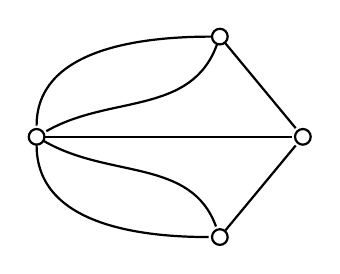
\begin{tikzpicture}[-,>=stealth,shorten >=1pt,auto,node distance=3cm,thick,main node/.style={scale=0.6,circle,draw,font=\sffamily\normalsize}]
            \node[main node] (1) {};
            \node[main node] (2) [below left of=1, xshift = -50] {};
            \node[main node] (3) [below right of=2, xshift = 50] {};
            \node[main node] (4) [right of=2, xshift = 75] {};

            \path[every node/.style={font=\sffamily\small}]
                (1) edge [out=180, in=90] (2)
                (1) edge [out=-110, in=30] (2)
                (2) edge [out=270, in=180] (3)
                (2) edge [out=-30, in=110] (3)
                (2) edge (4)
                (1) edge (4)
                (3) edge (4)
                ;
        \end{tikzpicture}
        \caption{The graph drawn by Euler which models the \tit{Seven Bridges of Königsberg} problem.}
        \label{konigsberg}
    \end{figure}

    Through his analysis, Euler discovered a fundamental rule: for a walk to cross each bridge exactly once and return to the starting point, every landmass had to be connected by an \tbf{even} number of bridges. In Königsberg's case, however, each landmass had an odd number of bridges, making the task impossible.

    Euler's proof, published in 1736, was groundbreaking --- not just because he solved the Königsberg puzzle, but because he laid the foundation for an entirely new branch of mathematics: \href{https://en.wikipedia.org/wiki/Graph_theory}{graph theory}. His ideas would go on to shape the study of networks, from modern transportation systems to social media connections and even the vast web of the internet itself. And so, from a simple question about bridges in a small Prussian city, a whole new field of mathematics was born—one that continues to shape the world centuries later.

    This chapter will discuss the basics of the field of \tbf{graph theory}, and will lay the foundation for later chapters.

    \section{Introduction}

    \begin{frameddefn}{Graph}
        A \tbf{graph} is a pair $G = (V, E)$, where $V$ is the --- finite --- set of \tbf{vertices} of the graph, and $E$ is the set of \tbf{edges}.
    \end{frameddefn}

    For now, will assume to be working with \tbf{simple} and \tbf{undirected} graphs, i.e. graphs in which the set of edges is defined as follows $$E \subseteq [V]^2 = \{\{x, y\} \mid x, y \in V \land x \neq v\}$$ where the notation $\{x, y\}$ will be used to indicate an edge between two nodes $x, y \in V$, and will be replaced with $xy = yx$ directly --- the \tit{set} notation for edges is used to highlight that edges have no direction.

    We will indicate with $n$ and $m$ the cardinality of $\abs V$ and $\abs E$, respectively. Moreover, we will indicate with $V(G)$ and $E(G)$ the set of the vertices and edges of $G$ respectively when there is ambiguity.

    \begin{figure}[H]
        \centering
        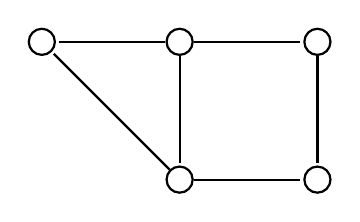
\begin{tikzpicture}[-,>=stealth,shorten >=1pt,auto,node distance=1.75cm, thick,main node/.style={scale=0.9,circle,draw,font=\sffamily\normalsize}]

            \node[circle, draw] (1) []{};
            \node[circle, draw] (2) [right of = 1]{};
            \node[circle, draw] (3) [below of = 1]{};
            \node[circle, draw] (4) [below of = 2]{};
            \node[circle, draw] (5) [left of = 1]{};

            \draw[-] (1) to (2);
            \draw[-] (1) to (3);
            \draw[-] (2) to (4);
            \draw[-] (1) to (5);
            \draw[-] (3) to (4);
            \draw[-] (3) to (5);

            ;
        \end{tikzpicture}
        \caption{A simple graph.}
        \label{first graph}
    \end{figure}

    Note that, in this definition, we are assuming that each edge has exactly 2 \tit{distinct} endpoints --- i.e. the graphs do not admit \tbf{loops} --- and there cannot be two edges with the same endpoints --- i.e. the graphs do not admit \tbf{parallel edges}. In fact, if we drop these assumption we obtain what is called a \tbf{multigraph}.

    \begin{figure}[H]
        \centering
        \begin{tikzpicture}[-,>=stealth',shorten >=1pt,auto,node distance=3cm,thick,main node/.style={scale=0.6,circle,draw,font=\sffamily\normalsize},every loop/.style={}]
            \node[main node] (1) {};
            \node[main node] (2) [below left of=1] {};
            \node[main node] (3) [below right of=2] {};

            \draw[-] (1) edge [bend left] (2);
            \draw[-] (1) edge [bend right](2);
            \draw[-] (2) edge (3);
            \draw[-] (3) edge (1);
            \draw[-] (3) edge [loop below] (3);

            ;
        \end{tikzpicture}
        \caption{A multigraph.}
    \end{figure}

    \begin{frameddefn}{Subgraph}
        Given a graph $G = (V, E)$, a \tbf{subgraph} $G' = (V', E')$ of $G$ is a graph such that $V' \subseteq V$ and $E' \subseteq E$. If $G'$ is a subgraph of $G$, then $G$ is called \tbf{supergraph} of $G'$.
    \end{frameddefn}

    \begin{figure}[H]
        \centering
        \begin{tikzpicture}[-,>=stealth,shorten >=1pt,auto,node distance=1.75cm, thick,main node/.style={scale=0.9,circle,draw,font=\sffamily\normalsize}]

            \node[circle, draw] (1) []{};
            \node[circle, draw] (2) [right of = 1]{};
            % \node[circle, draw] (3) [below of = 1]{};
            \node[circle, draw] (4) [below of = 2]{};
            \node[circle, draw] (5) [left of = 1]{};

            % \draw[-] (1) to (2);
            % \draw[-] (1) to (3);
            % \draw[-] (2) to (4);
            \draw[-] (1) to (5);
            % \draw[-] (3) to (4);
            % \draw[-] (3) to (5);

            ;
        \end{tikzpicture}
        \caption{This is a subgraph of the graph shown in \cref{first graph}.}
    \end{figure}

    \begin{frameddefn}{Induced subgraph}
        Given a graph $G = (V, E)$, a subgraph $G' = (V', E')$ of $G$ is \tbf{induced} if every edge of $G$ with both ends in $V$ is an edge of $V'$.
    \end{frameddefn}

    This definition is \tit{stricter} than the previous one: in fact, the last graph is \tit{not} an example of an induced subgraph, but the following is:

    \begin{figure}[H]
        \centering
        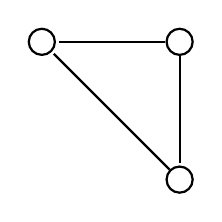
\begin{tikzpicture}[-,>=stealth,shorten >=1pt,auto,node distance=1.75cm, thick,main node/.style={scale=0.9,circle,draw,font=\sffamily\normalsize}]

            \node[circle, draw] (1) []{};
            % \node[circle, draw] (2) [right of = 1]{};
            \node[circle, draw] (3) [below of = 1]{};
            % \node[circle, draw] (4) [below of = 2]{};
            \node[circle, draw] (5) [left of = 1]{};

            % \draw[-] (1) to (2);
            \draw[-] (1) to (3);
            % \draw[-] (2) to (4);
            \draw[-] (1) to (5);
            % \draw[-] (3) to (4);
            \draw[-] (3) to (5);

            ;
        \end{tikzpicture}
        \caption{This is an \tit{induced} subgraph of the graph shown in \cref{first graph}.}
        \label{induced subgraph first graph}
    \end{figure}

    Note that every induced subgraph of a graph is \tbf{unique} by definition, and we indicate each induced subgraph as follows: suppose that the graph in \cref{first graph} had the following \tit{labeling} on the vertices

    \begin{figure}[H]
        \centering
        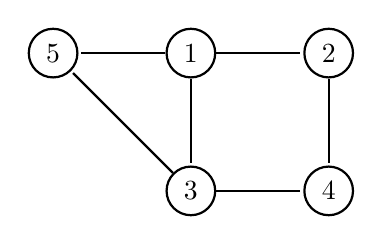
\begin{tikzpicture}[-,>=stealth,shorten >=1pt,auto,node distance=1.75cm, thick,main node/.style={scale=0.9,circle,draw,font=\sffamily\normalsize}]

            \node[circle, draw] (1) []{1};
            \node[circle, draw] (2) [right of = 1]{2};
            \node[circle, draw] (3) [below of = 1]{3};
            \node[circle, draw] (4) [below of = 2]{4};
            \node[circle, draw] (5) [left of = 1]{5};

            \draw[-] (1) to (2);
            \draw[-] (1) to (3);
            \draw[-] (2) to (4);
            \draw[-] (1) to (5);
            \draw[-] (3) to (4);
            \draw[-] (3) to (5);

            ;
        \end{tikzpicture}
        % \caption{This is an \tit{induced} subgraph of the graph shown in \cref{first graph}.}
    \end{figure}

    then, the induced subgraph in \cref{induced subgraph first graph} would have been referred to as $G[\{1, 3, 5\}]$.

    Intuitively, two vertices $x, y \in V$ are said to be \tbf{adjacent}, if there is an edge $xy \in E$, and we write $x \sim y$. If there is no such edge, we write $x \nsim y$ for non-adjacency. The \tbf{neighborhood} of a vertex $x \in V$ is the set of vertices that are adjacent to $x$, and it will be indicated as follows $$\mathcal N (x) := \{y \in V \mid x \sim y\}$$ Similarly, the neighborhood of a set of vertices will be defined as follows $$\forall S \subseteq V \quad \mathcal N(S) := \bigcup_{v \in S}{\mathcal N (v)}$$ The \tbf{degree} of a vertex $x \in V$, denoted with $\deg(x)$, is exactly $\abs{\mathcal N (x)}$. We will use the following notation for the \tbf{minimum} and \tbf{maximum} degree of a graph, respectively

    \begin{center}
        \begin{tabular}{ccc}
            $\displaystyle \delta := \min_{x \in V}{\deg(x)}$ & \qquad & $\displaystyle \Delta := \max_{x \in V}{\deg(x)}$
        \end{tabular}
    \end{center}

    \begin{framedlem}{Handshaking lemma}
        Given a graph $G = (V, E)$, it holds that $$\sum_{x \in V}{\deg(x)} = 2 \abs E$$
    \end{framedlem}

    \begin{proof}
        Trivially, the sum of the degrees counts every edge in $E$ exactly twice, once for each of the 2 endpoints.
    \end{proof}

    \begin{frameddefn}{$k$-regular graph}
        A graph $G$ is said to be \tbf{$k$-regular} if every vertex of $G$ has degree $k$.
    \end{frameddefn}

    Note that in a $k$-regular graph it holds that $$\sum_{x \in V}{\deg(x)} = k \cdot n$$

    \begin{framedprop}{}
        There are no $k$-regular graphs with $k$ odd and an odd number of vertices.
    \end{framedprop}
    
    \begin{proof}
        By way of contradiction, suppose that there exists a $k$-regular graph $G = (V, E)$ such that both $k$ and $n$ are odd; however, by the handshaking lemma we would get that $$2 \abs E = \sum_{x \in V} {\deg(x)} = k \cdot n$$ but the product of two odd numbers, namely $k$ and $n$, is still an odd number, while $2 \abs E$ must be even $\lightning$.
    \end{proof}

    \section{Important structures}

    \subsection{Paths, walks and cycles}

    \begin{frameddefn}{Path}
        A \tbf{path} is a \tit{graph} with vertex set $x_0, \ldots, x_n$ and edge set $e_1, \ldots, e_n$ such that $e_i = x_{i - 1}x_i$.

        The \tbf{length} of a path is the number of edges between $x_0$ and $x_n$, i.e. $\abs{\{e_1, \ldots, e_n\}}$, namely $n$ in this case. A path of length 1 is called \tit{trivial} path.
    \end{frameddefn}

    \begin{figure}[H]
        \centering
        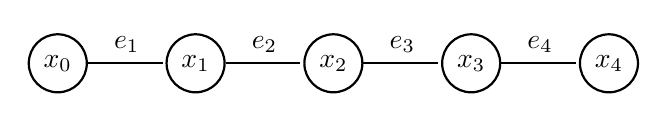
\begin{tikzpicture}[-,>=stealth,shorten >=1pt,auto,node distance=1.75cm, thick,main node/.style={scale=0.9,circle,draw,font=\sffamily\normalsize}]

            \node[circle, draw] (1) []{$x_0$};
            \node[circle, draw] (2) [right of = 1]{$x_1$};
            \node[circle, draw] (3) [right of = 2]{$x_2$};
            \node[circle, draw] (4) [right of = 3]{$x_3$};
            \node[circle, draw] (5) [right of = 4]{$x_4$};

            \draw[-] (1) to node[above]{$e_1$} (2);
            \draw[-] (2) to node[above]{$e_2$} (3);
            \draw[-] (3) to node[above]{$e_3$} (4);
            \draw[-] (4) to node[above]{$e_4$} (5);

            ;
        \end{tikzpicture}
        \caption{A path graph of length 4 that links $x_0$ and $x_4$.}
    \end{figure}

    Through \tit{paths} we can provide the definition of \tbf{distance} between two nodes of a graph.

    \begin{frameddefn}{Distance}
        Given a graph $G = (V, E)$, and two vertices $x, y \in V$, the \tbf{distance} between $x$ and $y$ in $G$, denoted with $\dist_G(x, y)$, is defined as the length of the \tit{shortest} path between $x$ and $y$ in $G$.
    \end{frameddefn}

    If there is no ambiguity, we will simply write $\dist(x, y)$ instead of $\dist_G(x, y)$. Finally, given a path $P$ and two vertices $u, v \in V(P)$, we will denote with $u \ P \ v$ the \tit{subpath} of $P$ between $u$ and $v$. Now, consider the following definition.

    \begin{frameddefn}{Walk}
        Given a graph $G = (V, E)$, a \tbf{walk} is a \tit{sequence} of vertices and edges $$x_0 \ e_1 \ x_1 \ \ldots \ x_{k - 1} \ e_k \ x_k$$ where $x_0, \ldots, x_k \in V$, $e_1, \ldots, e_k \in E$ and $e_i = x_{i - 1}x_i$.

        The \tbf{length} of a walk is the number of edges between $x_0$ and $x_k$, i.e. $\abs{\{e_1, \ldots , e_k \}}$, namely $k$ in this case. If $x_0 = x_k$ we say that the walk is \tbf{closed}.
    \end{frameddefn}

    If there is a path -- or a walk --- between two vertices $x, y \in V$, we say that the path --- or the walk --- \tbf{links} $x$ and $y$, and we write this as $x \to y$. Any vertex that is different from $x$ and $y$ is called \tit{internal node}. For instance, given the previous graph labeled as follows

    \begin{figure}[H]
        \centering
        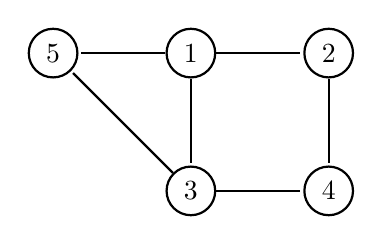
\begin{tikzpicture}[-,>=stealth,shorten >=1pt,auto,node distance=1.75cm, thick,main node/.style={scale=0.9,circle,draw,font=\sffamily\normalsize}]

            \node[circle, draw] (1) []{1};
            \node[circle, draw] (2) [right of = 1]{2};
            \node[circle, draw] (3) [below of = 1]{3};
            \node[circle, draw] (4) [below of = 2]{4};
            \node[circle, draw] (5) [left of = 1]{5};

            \draw[-] (1) to (2);
            \draw[-] (1) to (3);
            \draw[-] (2) to (4);
            \draw[-] (1) to (5);
            \draw[-] (3) to (4);
            \draw[-] (3) to (5);

            ;
        \end{tikzpicture}
        % \caption{Giv}
    \end{figure}

    an example of a walk over this graph is given by the following sequence $$1 \ \{1, 2\} \ 2 \ \{2, 4\} \ 4 \ \{4, 3\} \ 3 \ \{3, 1\} \ 1 \ \{1, 5\} \ 5$$ that \tit{links} 1 and 5, i.e. the walk is of the form $1 \to 5$.

    Note that there is a subtle difference between the definitions of \tbf{path} and \tbf{walk}: the definition of a path implies that this is always a \tit{graph} on its own, while a walk is defined as a \tit{sequence}. Nonetheless, we will treat \tit{paths} as if they where \tit{sequences} as well. This assumption holds for the following structures that will be discussed as well.

    However, by definition of path, not every alternating sequence of vertices and edges is a valid path, in fact:
    
    \begin{itemize}
        \item in a \tit{walk} it is possible to repeat both vertices and edges
        \item in a \tit{path} there can be no repetition of vertices nor edges (note that \tit{edge} repetition implies \tit{vertex} repetition)
    \end{itemize}

    For instance, the previous example of \tit{walk} is not a valid \tit{path}, because the vertex 1 is repeated.

    \begin{framedthm}[label={paths and walks}]{Paths and walks}
        Given a graph $G = (V, E)$ and two vertices $x, y \in V$, in $G$ there is a path $x \to y$ if and only if there is a walk $x \to y$.
    \end{framedthm}

    \begin{proof}
        By definition, every path is a walk, thus the direct implication is trivially true. To prove the converse implication, consider two vertices $x$ and $y$ for which there is at least one walk $x \to y$ in $G$. Now, out of all the possible walks $x \to y$ in $G$, consider the \tit{shortest} one, i.e. the one with the least amount of edges, and let it be the following sequence $$x \ e_1 \ x_1 \ \ldots \ x_{k - 1} \ e_k \ y $$ By way of contradiction, assume that this walk is not a path. Therefore, there must be either one vertex or one edge repeated, but since edge repetition always implies vertex repetition, we just need to take this case into account. Assume that there are two indices $i, j \in [k - 1]$ such that $i \neq j$ and $x_i = x_j$; however this implies that $$x \ e_1 \ \ldots \ x_{i - 1} \ e_i \ x_i \ e_{j + 1} \ x_{j + 1} \ \ldots \ x_{k - 1} \ e_k \ y$$ is still a walk $x \to y$ of strictly shorter length, but we chose the original sequence to be the \tit{shortest} possible walk $x \to y$ $\lightning$.
    \end{proof}

    \begin{framedprop}[label={longest path len}]{}
        The longest path in any graph has a length of at least $\delta$.
    \end{framedprop}
    
    \begin{proof}
        Consider a graph $G = (V, E)$, and let $P$ be a longest path in $G$, labeled as follows $$x_0 \ e_1 \ x_1 \ \ldots \ x_{k - 1} \ e_k \ x_k$$ and assume that its length is $k$. Since $P$ is a longest path in $G$, $x_k$ cannot have neighbors outside $P$ itself, otherwise $P$ would not have been the longest path of $G$ --- it could have been extended by one of $x_k$'s neighbors. This implies that $$\mathcal N(x_k) \subseteq \{x_0, \ldots, x_{k - 1}\}$$ and since $\delta \le \deg(x_k) := \abs{\mathcal N(x_k)}$ by definition of $\delta$, this implies that $$\delta \le \abs{\{x_0, \ldots, x_{k - 1}\}} = k$$
    \end{proof}

    \begin{frameddefn}{Cycle}
        A \tbf{cycle} is a \tit{graph} with vertex set $x_1, \ldots, x_n$ and edge set $x_1x_2, x_2x_3, \ldots, x_{n- 1}x_n, x_nx_1$.

        The \tbf{length} of a cycle is the number of edges between $x_1$ and $x_n$, namely $n$ in this case. A cycle of length $n$ is denoted as $C_n$.
    \end{frameddefn}

        \begin{figure}[H]
        \centering
        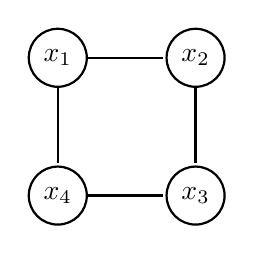
\begin{tikzpicture}[-,>=stealth,shorten >=1pt,auto,node distance=1.75cm, thick,main node/.style={scale=0.9,circle,draw,font=\sffamily\normalsize}]

            \node[circle, draw] (1) []{$x_1$};
            \node[circle, draw] (2) [right of = 1]{$x_2$};
            \node[circle, draw] (3) [below of = 1]{$x_4$};
            \node[circle, draw] (4) [below of = 2]{$x_3$};

            \draw[-] (1) to (2);
            \draw[-] (1) to (3);
            \draw[-] (2) to (4);
            \draw[-] (3) to (4);

            ;
        \end{tikzpicture}
        \caption{A cycle graph of length 4.}
    \end{figure}

    A graph that does not admit cycle subgraphs --- or \tit{cycles}, for short --- is said to be \tbf{acyclic}.

    \begin{framedprop}[label={min deg 2}]{}
        Every graph with $\delta \ge 2$ has a cycle of length at least $\delta + 1$.
    \end{framedprop}

    \begin{proof}
        Consider the proof of \cref{longest path len}; by applying the same reasoning, we know that $x_k$ cannot have neighbors outside $P$ itself. However, since $\delta \ge 2$, and $x_k \sim x_{k - 1}$, there must be at least one vertex in $x_k$'s neighborhood that lies in $P$. Therefore, let $x_i$ be the first vertex of $P$ --- w.r.t. our labeling of $P$ --- that is adjacent to $x_k$; hence, we have $$\mathcal N (x_k) \subseteq \{x_i, \ldots, x_{k - 1}\} \implies \delta \le \abs{\{x_i, \ldots, x_{k - 1}\}}$$ which implies that $x_i, \ldots, x_{k - 1}, x_k, x_i$ is a cycle of length at least $\delta + 1$.
    \end{proof}

    \begin{frameddefn}{Connected graph}
        An undirected graph $G = (V, E)$ is said to be \tbf{connected} if and only if for each vertex pair $x, y \in V$ there is a path $x \to y$.
    \end{frameddefn}

    All the graphs that we presented so far are \tit{connected}, thus the following figure provides an example of an \tbf{disconnected} graph.

    \begin{figure}[H]
        \centering
        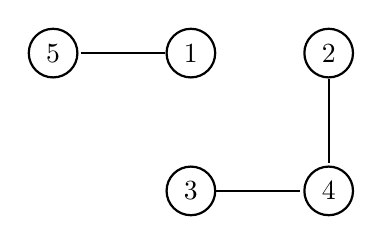
\begin{tikzpicture}[-,>=stealth,shorten >=1pt,auto,node distance=1.75cm, thick,main node/.style={scale=0.9,circle,draw,font=\sffamily\normalsize}]

            \node[circle, draw] (1) []{1};
            \node[circle, draw] (2) [right of = 1]{2};
            \node[circle, draw] (3) [below of = 1]{3};
            \node[circle, draw] (4) [below of = 2]{4};
            \node[circle, draw] (5) [left of = 1]{5};

            % \draw[-] (1) to (2);
            % \draw[-] (1) to (3);
            \draw[-] (2) to (4);
            \draw[-] (1) to (5);
            \draw[-] (3) to (4);
            % \draw[-] (3) to (5);

            ;
        \end{tikzpicture}
        % \caption{An disconnected graph.}
    \end{figure}

    \begin{frameddefn}{Component}
        Given a graph $G$, a \tbf{component} of $G$ is a maximal connected subgraph of $G$.
    \end{frameddefn}

    For instance, the graph of the previous example is made up of 2 components, namely the following two subgraphs $$C_1 = (\{1, 5\}, \{\{1, 5\}\})$$ $$C_2 = (\{2, 3, 4\}, \{\{2, 4\}, \{4, 3\}\})$$

    \begin{framedprop}[label={avoid cycle}]{}
        If $G$ is a connected graph, and $C$ is a cycle in $G$, then for any edge $e \in C$ it holds that $G - \{e\}$ is still connected.
    \end{framedprop}

    \begin{proof}
        Consider a graph $G = (V, E)$ that has a cycle $C$, and any two vertices $x, y \in V$; in particular, since $G$ is connected, there must be a path $x \to y$ in $G$, and let this path be $$P = x \ e_1 \ x_1 \ \ldots \ x_{k - 1} \ e_k \ y$$ Consider an edge $e \in C$; if $P$ does not traverse $e$, trivially $G - \{e\}$ will still contain $P$.

        Now let $$C = z_1 \ f_2 \ z_2 \ \ldots \ z_{l- 1} \ f_l \ z_l \ f_{l + 1} \ z_1$$ and without loss of generality assume that $e = f_2 = z_1 z_2 = x_i x_{i + 1} = e_{i + 1}$ for some $i \in [k - 1]$. Thus we can construct the following walk $$x \ e_1 \ x_1 \ \ldots \ x_i \ f_{l + 1} \ z_l \ \ldots \ f_3 \ z_2 \ e_{i + 2} \ x_{i + 2} \ \ldots \ x_{k - 1} \ e_k \ y$$ from $x$ to $y$, and by \cref{paths and walks} we have that there is a path from $x \to y$, which proves that $G - \{e\}$ is still connected.
    \end{proof}

    \subsection{Trees}

    \begin{frameddefn}{Tree}
        A \tbf{tree} is a connected acyclic graph. Usually, but not necessarily, there is a fixed vertex called \tbf{root}, and any vertex that has degree 1 in the tree is called \tbf{leaf}.
    \end{frameddefn}
    
    \begin{figure}[H]
        \centering
        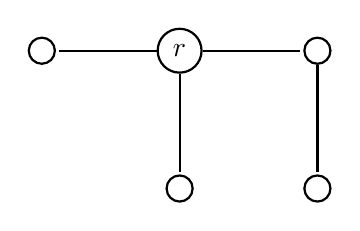
\begin{tikzpicture}[-,>=stealth,shorten >=1pt,auto,node distance=1.75cm, thick,main node/.style={scale=0.9,circle,draw,font=\sffamily\normalsize}]

            \node[circle, draw] (1) []{$r$};
            \node[circle, draw] (2) [right of = 1]{};
            \node[circle, draw] (3) [below of = 1]{};
            \node[circle, draw] (4) [below of = 2]{};
            \node[circle, draw] (5) [left of = 1]{};

            \draw[-] (1) to (2);
            \draw[-] (1) to (3);
            \draw[-] (2) to (4);
            \draw[-] (1) to (5);
            % \draw[-] (3) to (4);
            % \draw[-] (3) to (5);

            ;
        \end{tikzpicture}
        \caption{A tree with tree leaves, rooted in $r$.}
    \end{figure}

    A \tbf{forest} is an disconnected graph in which each component is a \tit{tree}, as in the following example

    \begin{figure}[H]
        \centering
        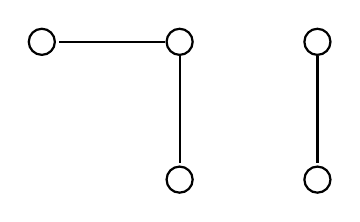
\begin{tikzpicture}[-,>=stealth,shorten >=1pt,auto,node distance=1.75cm, thick,main node/.style={scale=0.9,circle,draw,font=\sffamily\normalsize}]

            \node[circle, draw] (1) []{};
            \node[circle, draw] (2) [right of = 1]{};
            \node[circle, draw] (3) [below of = 1]{};
            \node[circle, draw] (4) [below of = 2]{};
            \node[circle, draw] (5) [left of = 1]{};

            % \draw[-] (1) to (2);
            \draw[-] (1) to (3);
            \draw[-] (2) to (4);
            \draw[-] (1) to (5);
            % \draw[-] (3) to (4);
            % \draw[-] (3) to (5);

            ;
        \end{tikzpicture}
        \caption{A forest.}
    \end{figure}

    Given a tree $T$ rooted in some node $r \in V(T)$, and two vertices $x, y \in V(T)$, consider the paths $P_x$ of the form $x \to r$ and $P_y$ of the form $y \to r$, respectively. The first vertex of $P_y$ that is encountered by tracing $P_x$ from $x$ to $r$ is called \tbf{lowest common ancestor} (LCA) of $x$ and $y$.

    \begin{figure}[H]
        \centering
        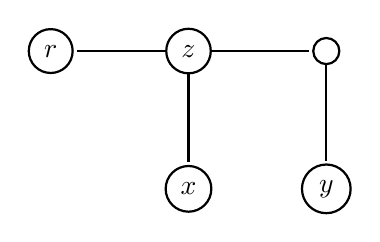
\begin{tikzpicture}[-,>=stealth,shorten >=1pt,auto,node distance=1.75cm, thick,main node/.style={scale=0.9,circle,draw,font=\sffamily\normalsize}]

            \node[circle, draw] (1) []{$z$};
            \node[circle, draw] (2) [right of = 1]{};
            \node[circle, draw] (3) [below of = 1]{$x$};
            \node[circle, draw] (4) [below of = 2]{$y$};
            \node[circle, draw] (5) [left of = 1]{$r$};

            \draw[-] (1) to (2);
            \draw[-] (1) to (3);
            \draw[-] (2) to (4);
            \draw[-] (1) to (5);
            % \draw[-] (3) to (4);
            % \draw[-] (3) to (5);

            ;
        \end{tikzpicture}
        \caption{For instance, in this tree --- rooted in $r$ --- the LCA of $x$ and $y$ is the vertex labeled with $z$.}
    \end{figure}

    Note that the LCA between any two vertices of a tree is \tit{always defined}, since in the \curlyquotes{worst case} it is the root $r$ itself.

    \begin{framedthm}[label={tree alt}]{Alternative definitions of tree}
        Given a graph $T = (V, E)$, the following statements are equivalent:

        \begin{enumerate}
            \item $T$ is a tree
            \item every vertex pair of $T$ is connected by a unique path
            \item $T$ is \tit{minimally connected}, i.e. $T$ is connected and $\forall e \in E$ it holds that $T- \{e\}$ is disconnected
            \item $T$ is \tit{maximally acyclic}, i.e. $T$ is acyclic and $\forall x, y \in V$ such that $x \nsim y$, it holds that $T \cup \{xy\}$ has a cycle
        \end{enumerate}
    \end{framedthm}

    \begin{proof}
        We will prove the statements cyclically.
        \begin{itemize}
            \item $1 \implies 2$. By contrapositive, assume that in $T$ there exist two vertices $x, y \in V$ for which there are two distinct paths $P$ and $Q$ of the form $x \to y$. If $P$ and $Q$ are edge-disjoint, then $P \cup Q$ is a cycle, which implies that $T$ is not a tree by definition.

                Otherwise, assume that $P$ and $Q$ are not edge-disjoint. If we start say in $x$, and we follow $Q$ edge by edge since $P$ and $Q$ are distinct, at some point we will encounter an edge $\{u, v\}$ such that $u \in P \cap Q$ and $v \in Q - P$ --- possibly, $u = x$ itself. Moreover, since both paths lead to $y$, if we keep following $Q$ we will encounter a vertex $z \in P \cap Q$ --- possibly, $z = y$ itself --- from which the two paths will coincide. Let $Q'$ be the subpath of $P$ starting with $u$ and ending in $z$; then, $Q' \cup (Q - P)$ is a cycle in $T$, which implies that $T$ is not a tree by definition.

                \begin{figure}[H]
                    \centering
                    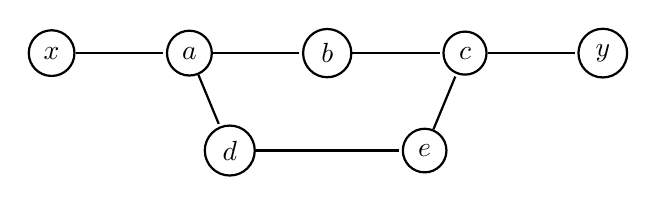
\begin{tikzpicture}[-,>=stealth,shorten >=1pt,auto,node distance=1.75cm, thick,main node/.style={scale=0.9,circle,draw,font=\sffamily\normalsize}]

                        \node[circle, draw] (1) []{$x$};
                        \node[circle, draw] (2) [right of = 1]{$a$};
                        \node[circle, draw] (3) [right of = 2]{$b$};
                        \node[circle, draw] (4) [right of = 3]{$c$};
                        \node[circle, draw] (5) [right of = 4]{$y$};
                        \node[circle, draw] (6) [below left of = 3]{$d$};
                        \node[circle, draw] (7) [below right of = 3]{$e$};

                        \draw[-] (1) to (2);
                        \draw[-] (2) to (3);
                        \draw[-] (3) to (4);
                        \draw[-] (4) to (5);
                        \draw[-] (2) to (6);
                        \draw[-] (7) to (4);
                        \draw[-] (6) to (7);

                        ;
                    \end{tikzpicture}
                    \caption{For instance, applying the argument of the proof in this graph we would get that $P = \{x, a, b, c, y\}$, $Q = \{x, a, d, e, c, y\}$, $Q - P = \{d, e\}$, $u = a$, $z = c$ and $Q' = \{a, b, c\}$, in fact $Q' \cup (Q - P) = \{a, b, c, e, d\}$ which is a cycle.}
                \end{figure}
            \item $2 \implies 3$. Consider an edge $xy \in E$; this edge itself is a path $x \to y$, and if we assume statement 2 this implies that it is the \tit{only} path from $x$ to $y$. This implies that $T - \{xy\}$ cannot contain a path from $x$ to $y$, therefore $T - \{xy\}$ is disconnected.
            \item $3 \implies 4$. Since statement 3 implies that $T$ is connected, by \cref{avoid cycle} we have that $T$ is acyclic. Now, pick $x, y \in V$ such that $x \nsim y$; by connectivity of $T$ there must be a path $x \to y$ in $T$, and let this path be $P$. Lastly, since $x \nsim y$, we have that $P \cup \{xy\}$ is a cycle in $T$.
            \item $4 \implies 1$ By contrapositive, we want to prove that if $T$ is not a tree, then $T$ is not maximally acyclic. Note that if $T$ is not a tree, we have two options:

                \begin{itemize}
                    \item if $T$ is connected but contains a cycle, then $T$ is clearly not maximally acyclic
                    \item if $T$ is acyclic but disconnected, then by definition there must be two vertices $x, y \in V$ such that there is no path $x \to y$, which implies that $T \cup \{xy\}$ still does not contain any cycle
                \end{itemize}
        \end{itemize}
    \end{proof}

    \begin{framedlem}[label={leaf existence}]{}
        Every tree with at least 2 vertices has a leaf.
    \end{framedlem}
    
    \begin{proof}
        By way of contradiction, assume $T$ is a tree with at least 2 vertices that does not contain any leaves; then $\delta \ge 2$ in $T$, which implies that $T$ contains a cycle of length at least $\delta + 1$ by \cref{min deg 2}.
    \end{proof}

    \begin{framedlem}[label={tree without leaf}]{}
        Given a tree $T$, and a leaf $v$ of $T$, it holds that $T - \{v\}$ is still a tree.
    \end{framedlem}

    \begin{proof}
        Since $T$ is acyclic by definition, $T - \{v\}$ is still acyclic, we just need to prove that $T - \{v\}$ is still connected. By way of contradiction, assume that in $T - \{v\}$ there exist two vertices $x$ and $y$ such that there is no path between them. However, since $T$ is connected, there is a path $P$ of the form $x \to y$ in $T$.

        Note that, if by removing $v$ from $T$ we disconnect $x$ and $y$, it must be that $v$ lies in $P$. Moreover, since $v$ is in $T$ but not in $T - \{v\}$, while both $x$ and $y$ are also in $T - \{v\}$, it must be that $v$ is an \tit{internal} node of $P$, i.e. $v \neq x, y$, which implies that $\deg(v) \ge 2$ by definition of path, contradicting the hypothesis for which $v$ was a leaf $\lightning$.
    \end{proof}

    \begin{framedprop}[label={m n - 1}]{}
        If $T$ is a tree, then $m = n - 1$.
    \end{framedprop}

    \proofind{
        We will prove the statement by induction on $n$
    }{
        When $n = 1$, there are no edges in the tree, and $0 = m = 1 - 1$.
    }{
        Assume that for a tree that has $n = k - 1$ nodes the statement holds.
    }{
        We will prove the statement for a tree $T$ that has $n = k$ nodes. Note that, since $n = 1$ is the base case, we can assume that $n = k \ge 2$, hence by \cref{leaf existence} $T$ contains at least one leaf. Let this leaf be $v$; then, by \cref{tree without leaf} it holds that $T - \{v\}$ is still a tree, and clearly $T - \{v\}$ has $k - 1$ nodes, which implies that we can apply the inductive hypothesis on $T - \{v\}$, i.e. $$\abs{E(T - \{v\})} = \abs{V(T - \{v\})} - 1 = k - 1 - 1 = k - 2$$ However, note that $v$ is a leaf, concluding that $$m = \abs{E(T)} = \abs{E(T - \{v\})} + 1 = k - 2 + 1 = k - 1 = n - 1$$
    }

    \begin{frameddefn}{Spanning tree}
        Given a graph $G = (V, E)$, a \tbf{spanning tree} $T$ of $G$ is a subgraph of $G$ such that

        \begin{itemize}
            \item $T$ is a tree
            \item $V(T) = V(G)$, i.e. $T$ \tit{spans} every vertex of $G$
        \end{itemize}
    \end{frameddefn}

    For instance, given the graph in \cref{first graph}, a possible spanning tree is the following:

    \begin{figure}[H]
        \centering
        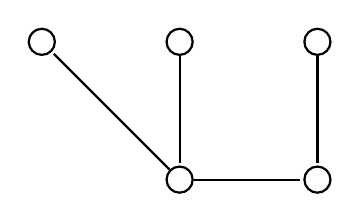
\begin{tikzpicture}[-,>=stealth,shorten >=1pt,auto,node distance=1.75cm, thick,main node/.style={scale=0.9,circle,draw,font=\sffamily\normalsize}]

            \node[circle, draw] (1) []{};
            \node[circle, draw] (2) [right of = 1]{};
            \node[circle, draw] (3) [below of = 1]{};
            \node[circle, draw] (4) [below of = 2]{};
            \node[circle, draw] (5) [left of = 1]{};

            % \draw[-] (1) to (2);
            \draw[-] (1) to (3);
            \draw[-] (2) to (4);
            % \draw[-] (1) to (5);
            \draw[-] (3) to (4);
            \draw[-] (3) to (5);

            ;
        \end{tikzpicture}
        % \caption{A tree with tree leaves.}
    \end{figure}

    \begin{framedlem}[label={spanning tree existence}]{}
        Any connected graph has a spanning tree.
    \end{framedlem}

    \begin{proof}
        Consider a connected graph $G$, and keep removing edges from $E(G)$ --- and their relative endpoints from $V(G)$ --- one by one, as long as $G$ is still connected. If no other edge can be removed from $G$ without violating connectivity, we will end up with a graph that must be a tree by statement 3 of \cref{tree alt}.
    \end{proof}

    Thanks to this last proposition, we can actually prove a stronger version of the \cref{m n - 1}, which is the following.

    \begin{framedthm}{}
        $T$ is a tree if and only if $T$ is connected and $m = n - 1$.
    \end{framedthm}

    \begin{proof}
        The direct implication is proved in \cref{m n - 1}, so we just need to prove the converse implication. Consider a connected graph $T$ such that $m = n - 1$; by \cref{spanning tree existence} $T$ must have a spanning tree $T'$, and by \cref{m n - 1} itself it holds that $\abs{E(T')} = \abs{V(T')} - 1$. However, $T'$ is a spanning tree of $T$, therefore $$V(T) = V(T') \implies \abs{V(T)} = \abs{V(T')} \implies \abs{E(T')} = \abs{V(T)} - 1 = \abs{E(T)}$$ which implies $E(T) = E(T')$ because $T'$ is a subgraph of $T$, therefore $T = T'$, concluding that $T$ must be a tree since $T'$ is a tree.
    \end{proof}

    \subsection{Bipartite graphs}

    \begin{frameddefn}{Bipartite graph}
        A graph $G = (V, E)$ is said to be \tbf{bipartite} if there exists a set $X \subseteq V$ such that every edge of $G$ has exactly one endpoint in $X$ and one in $V - X$. If such a set $X$ exists, we say that $(X, V - x)$ is a \tbf{bipartition} of $G$.
    \end{frameddefn}

    \begin{figure}[H]
        \centering
        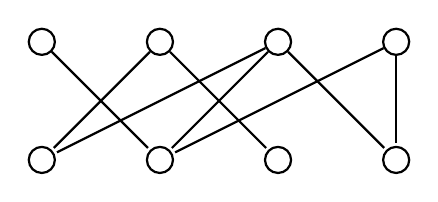
\begin{tikzpicture}[-,>=stealth,shorten >=1pt,auto,node distance=1.5cm, thick,main node/.style={scale=0.9,circle,draw,font=\sffamily\normalsize}]

            \node[circle, draw] (1) []{};
            \node[circle, draw] (2) [right of = 1]{};
            \node[circle, draw] (3) [right of = 2]{};
            \node[circle, draw] (4) [right of = 3]{};
            \node[circle, draw] (5) [below of = 1]{};
            \node[circle, draw] (6) [below of = 2]{};
            \node[circle, draw] (7) [below of = 3]{};
            \node[circle, draw] (8) [below of = 4]{};

            \draw[-] (1) to (6);
            \draw[-] (2) to (5);
            \draw[-] (2) to (7);
            \draw[-] (3) to (5);
            \draw[-] (3) to (6);
            \draw[-] (3) to (8);
            \draw[-] (4) to (6);
            \draw[-] (4) to (8);

            ;
        \end{tikzpicture}
        \caption{An example of a \tit{bipartite graph}. In particular, if we call the uppermost set of nodes $A$ and the lowermost one $B$, then $(A, B)$ is a bipartition of the graph.}
        % \label{}
    \end{figure}

    There are various types of graphs that can be bipartitioned. For example, any \tbf{tree} $T$ can be bipartitioned through a bipartition $(X, V(T) - X)$ by considering the following set of vertices $$X := \{v \in V(T) \mid \dist(r, v) \ \mathrm{even}\}$$ where $r$ is $T$'s root.

    \begin{figure}[H]
        \centering
        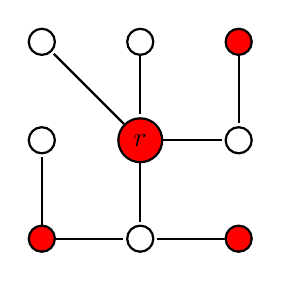
\begin{tikzpicture}[-,>=stealth,shorten >=1pt,auto,node distance=1.25cm, thick,main node/.style={scale=0.9,circle,draw,font=\sffamily\normalsize}]

            \node[circle, draw] (1) []{};
            \node[circle, draw, fill=red] (2) [right of = 1]{};
            \node[circle, draw, fill=red] (3) [below of = 1]{$r$};
            \node[circle, draw] (4) [below of = 2]{};
            \node[circle, draw] (5) [left of = 1]{};
            \node[circle, draw] (6) [below of = 3]{};
            \node[circle, draw, fill=red] (7) [right of = 6]{};
            \node[circle, draw, fill=red] (8) [left of = 6]{};
            \node[circle, draw] (9) [above of = 8]{};

            % \draw[-] (1) to (2);
            \draw[-] (1) to (3);
            \draw[-] (2) to (4);
            % \draw[-] (1) to (5);
            \draw[-] (3) to (4);
            \draw[-] (3) to (5);
            \draw[-] (3) to (6);
            \draw[-] (7) to (6);
            \draw[-] (8) to (6);
            \draw[-] (8) to (9);

            ;
        \end{tikzpicture}
        \caption{The set of red vertices $X$ defines a bipartition $(X, V(T) - X)$ of this tree $T$.}
    \end{figure}

    However, \tit{not every type} of graph can be bipartitioned. For instance, consider the following type.

    \begin{frameddefn}{Clique}
        A \tbf{clique} is a \tit{graph} in which each vertex is adjacent to any other vertex of the graph. A clique that has $n$ vertices is denoted as $K_n$.
    \end{frameddefn}

    \begin{figure}[H]
        \centering
        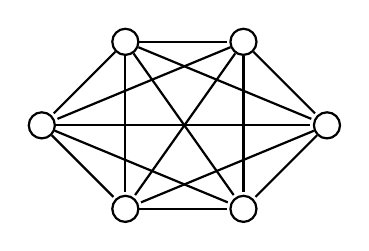
\begin{tikzpicture}[-,>=stealth,shorten >=1pt,auto,node distance=1.5cm, thick,main node/.style={scale=0.9,circle,draw,font=\sffamily\normalsize}]

            \node[circle, draw] (1) []{};
            \node[circle, draw] (2) [right of = 1]{};
            \node[circle, draw] (3) [below left of = 1]{};
            \node[circle, draw] (4) [below right of = 2]{};
            \node[circle, draw] (5) [below right of = 3]{};
            \node[circle, draw] (6) [below left of = 4]{};

            \draw[-] (1) to (2);
            \draw[-] (1) to (3);
            \draw[-] (1) to (4);
            \draw[-] (1) to (5);
            \draw[-] (1) to (6);
            \draw[-] (2) to (3);
            \draw[-] (2) to (4);
            \draw[-] (2) to (5);
            \draw[-] (2) to (6);
            \draw[-] (3) to (4);
            \draw[-] (3) to (5);
            \draw[-] (3) to (6);
            \draw[-] (4) to (5);
            \draw[-] (4) to (6);
            \draw[-] (5) to (6);

            ;
        \end{tikzpicture}
        \caption{The clique $K_6$.}
        % \label{}
    \end{figure}

    It is easy to see that no clique $K_n$ can be bipartitioned, since there is an edge between any pair of vertices of the graph. However, this is not the only type of graph that cannot be bipartitioned.

    \begin{framedlem}{}
        If $G$ is a bipartite graph, and $H$ is a subgraph of $G$, then $H$ must be bipartite.
    \end{framedlem}
    
    \begin{proof}
        Given a bipartite graph $G = (V, E)$, assume that $(X, V - X)$ is a bipartition of $G$, and let $H$ be a subgraph of $G$; then, it is easy to see that $(X \cap V(H), V(H) - X)$ is a bipartition for $H$.
    \end{proof}

    Note that this lemma implies that $G$ is bipartite if and only if every connected component of $G$ is bipartite: in fact, the direct implication follows from this lemma, and the following figure provides an intuition for the converse implication.

        \begin{figure}[H]
        \centering
        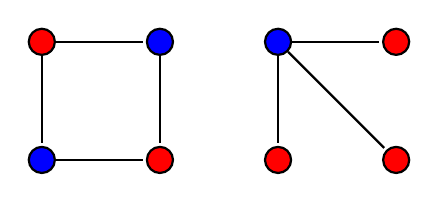
\begin{tikzpicture}[-,>=stealth,shorten >=1pt,auto,node distance=1.5cm, thick,main node/.style={scale=0.9,circle,draw,font=\sffamily\normalsize}]

            \node[circle, draw, fill=red] (1) []{};
            \node[circle, draw, fill=blue] (2) [right of = 1]{};
            \node[circle, draw, fill=blue] (3) [below of = 1]{};
            \node[circle, draw, fill=red] (4) [right of = 3]{};
            \node[circle, draw, fill=blue] (5) [right of = 2]{};
            \node[circle, draw, fill=red] (6) [right of = 5]{};
            \node[circle, draw, fill=red] (7) [below of = 5]{};
            \node[circle, draw, fill=red] (8) [right of = 7]{};

            \draw[-] (1) to (2);
            \draw[-] (1) to (3);
            \draw[-] (2) to (4);
            \draw[-] (3) to (4);

            \draw[-] (5) to (6);
            \draw[-] (5) to (7);
            \draw[-] (5) to (8);

            ;
        \end{tikzpicture}
        \caption{Consider the following disconnected graph $G$ made of these two connected components, $C_1$ and $C_2$ respectively. Say that $C_1$ has a bipartition $(X_1, V(C_1) - X_1)$ where $X_1$ is the red set, and $C_2$ has a bipartition $(X_2, V(C_2) - X_2)$ where $X_2$ is the red set; thus, $(X_1 \cup X_2, V(C_1 \cup C_2) - X_1 - X_2)$ is clearly a bipartition of $G$. This process may be repeated for all the connected components of any disconnected graph.}
        % \label{}
    \end{figure}

    \begin{framedthm}{Bipartite graphs}
        $G$ is bipartite if and only if $G$ has no odd-length cycle.
    \end{framedthm}

    \proofiff{
        We will prove the contrapositive, i.e. if $G$ has an odd-length cycle, then $G$ cannot be bipartitioned. Consider a graph $G$ with an odd-length cycle $C_{2k + 1}$ of vertices $x_1, \ldots, x_{2k + 1}$; by way of contradiction, assume that $G$ is bipartite through a bipartition $(X, V(G)) - X)$ for some $X \subseteq V(G)$. Without loss of generality assume that $x_1 \in X$; then, since $X$ defines a bipartition of $G$ it must be that $x_2 \notin X$, and $x_3 \in X$ and so on and so forth. In particular, for any odd value of $i$ we will have that $x_i \in X$, but this implies that both $x_1$ and $x_{2k + 1}$ must be inside $X$, which means that the edge $x_1x_{2k + 1}$ violates the bipartition induced by $X$ $\lightning$.
    }{
        Again, we will prove the contrapositive, i.e. if $G$ is not bipartite it must contain an odd-length cycle. By the previous observation, $G$ is not bipartite if and only if at least one connected component of $G$ is not bipartite, and let this component be $\overline G$. Note that, since $\overline G$ is connected, it must contain a spannning tree $T$ by \cref{spanning tree existence}. Moreover, as previously described, we can always define a bipartition on a tree, namely $(X, V(T) - X)$ where $$\textstyle X := \{v \in V(T) \mid \dist_T(r, v) \ \mathrm{even}\}$$ for some root node $r \in V(T)$.

        Now, since $T$ is a spanning tree of $\overline G$, which is now bipartite by hypothesis, there must be an edge $xy \in V(\overline G)$ such that either $x, y \in X$ or $x, y \in V(T) - X$, i.e. the edge $xy$ must have both endpoints in the same set of $T$'s bipartition. Let $z$ be the LCA between $x$ and $y$ in $T$, and $P_x$ and $P_y$ be the paths of the form $x \to r$ and $y \to r$, respectively. Note that, since $xy$ has both endpoints in the same set, it must be that the lengths of $P_x$ and $P_y$ have the same parity by definition of $X$. Lastly, by statement 2 of \cref{tree alt} we have that $r \ P_x \ z = r \ P_y \ z$, which implies that the lengths of $z \ P_x \ x$ and $z \ P_y \ y$ must have the same parity. This concludes that $$z \ P_x \ x \cup z \ P_y \ y \cup xy$$ is an odd-length cycle of $G$.
    }

    \subsection{Eulerian tours}

    At the start of this chapter, we introduced the \tit{Seven Bridges of Königsberg} problem, which led to the emergence of graph theory as a branch of combinatorics. Over time, as the field developed, this problem was formalized into the following definition.

    \begin{frameddefn}{Eulerian tour}
        An \tbf{Eulerian tour} over a graph $G$ is a closed walk that traverses every edge of $G$ exactly once.
    \end{frameddefn}

    For instance, consider the following graph

    \begin{figure}[H]
        \centering
        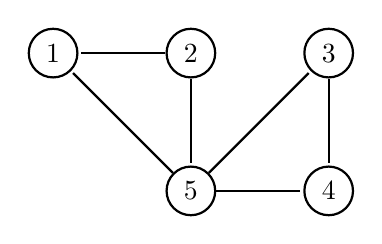
\begin{tikzpicture}[-,>=stealth,shorten >=1pt,auto,node distance=1.75cm, thick,main node/.style={scale=0.9,circle,draw,font=\sffamily\normalsize}]

            \node[circle, draw] (1) []{2};
            \node[circle, draw] (2) [right of = 1]{3};
            \node[circle, draw] (3) [below of = 1]{5};
            \node[circle, draw] (4) [below of = 2]{4};
            \node[circle, draw] (5) [left of = 1]{1};

            \draw[-] (3) to (2);
            \draw[-] (1) to (3);
            \draw[-] (2) to (4);
            \draw[-] (1) to (5);
            \draw[-] (3) to (4);
            \draw[-] (3) to (5);

            ;
        \end{tikzpicture}
        % \caption{A simple graph.}
        % \label{first graph}
    \end{figure}

    After some trial an error, it is easy to find an Eulerian tour over this graph, for instance $$1 \ \{1, 2\} \ 2 \ \{2, 5\} \ 5 \ \{5, 3\} \ 3 \ \{3, 4\} \ 4 \ \{4, 5\} \ 5 \ \{5, 1\} \ 1$$ Note that this is a valid Eulerian tour because there is no edge repetition, and vertex repetition is allowed by definition. On the counter side, the graph --- or, more precisely, the \tit{multigraph} --- that the bridges of Königsberg define, which is the following

    \begin{figure}[H]
        \centering
        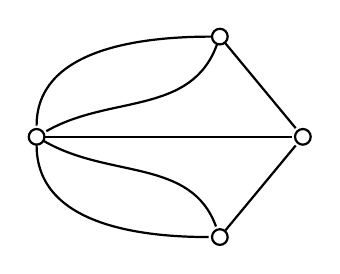
\begin{tikzpicture}[-,>=stealth,shorten >=1pt,auto,node distance=3cm,thick,main node/.style={scale=0.6,circle,draw,font=\sffamily\normalsize}]
            \node[main node] (1) {};
            \node[main node] (2) [below left of=1, xshift = -50] {};
            \node[main node] (3) [below right of=2, xshift = 50] {};
            \node[main node] (4) [right of=2, xshift = 75] {};

            \path[every node/.style={font=\sffamily\small}]
                (1) edge [out=180, in=90] (2)
                (1) edge [out=-110, in=30] (2)
                (2) edge [out=270, in=180] (3)
                (2) edge [out=-30, in=110] (3)
                (2) edge (4)
                (1) edge (4)
                (3) edge (4)
                ;
        \end{tikzpicture}
        % \caption{The graph drawn by Euler which models the \tit{Seven Bridges of Königsberg} problem.}
        % \label{konigsberg}
    \end{figure}

    does not admit any Eulerian tour. But, given a graph, how can we determine with certainty whether it contains an Eulerian tour? The following theorem, proved by Euler himself in his original paper \cite{konigsberg}, answers this question. Note that this theorem holds both for graphs and multigraph.

    \begin{framedthm}{Eulerian tours}
        A graph $G$ admits an Eulerian tour if and only $G$ is connected and every vertex of $G$ has even degree.
    \end{framedthm}
    
    \proofiff{
        Consider the contrapositive of the direct implication, and assume that $G$ contains at least one odd-degree vertex $v$. Recall that an Eulerian tour is a closed walk that does not allow edge repetition, which implies that the \tit{starting} point of the walk is actually not relevant. Therefore, we can assume without loss of generality that any possible Eulerian tour defined on $G$ starts on $v$ itself, but then to be \tit{closed} it must end on $v$ as well. Moreover, each time any Eulerian tour passes through $v$ it must use 2 distinct edges, however $v$ is an odd-degree vertex, therefore at the end of the Eulerian tour there is no way we can come back to $v$ and close the walk.
    }{
        Consider a graph $G$ in which every vertex has even degree, and let $W$ be the \tit{longest} walk of $G$ that does not repeat edges, and let it be labeled as follows $$x_0 \ e_1 \ x_1 \ \ldots \ x_{k - 1} \ e_k \ x_k$$ 

        \claim{
            $x_0 = x_k$, i.e. $W$ is closed.
        }{
            By way of contradiction, assume that $W$ $x_0 \neq x_k$. If this is the case, then $x_k = v$ for some vertex $v$ that is not $x_0$. Note that $W$ is a \tit{walk}, therefore $v$ may be repeated multiple times inside $W$, i.e. $$x_0 \ e_1 \ x_1 \ \ldots \ v \ \ldots \ v \ \ldots \ x_{k - 1} \ e_k \ v$$ If $l$ is the number of times $v$ occurs in $W$ \tit{without counting} $x_k$, then clearly in $W$ there are $2l + 1$ edges incident to $v$, namely $e_k$ and 2 edges each other time $v$ appears in $W$. However, since $2l + 1$ is odd and we assumed that $G$ has no odd-degree vertices, there must be at least one edge $vu \in E(G)$ such that $u \notin V(W)$. This implies that $$x_0 \ e_1 \ x_1 \ \ldots \ x_{k - 1} \ e_k \ v \ vu \ u$$ is a longer walk than $W$, and it does not repeat any edges because $uv \notin E(W)$, contradicting the definition of $W$ $\lightning$.
        }

        This claim proves that $W$ is closed, but we still need to prove that it traverses every edge to claim that it is indeed an Eulerian tour. By way of contradiction, assume that there exists at least one edge $e \notin E(W)$ not used by $W$. Consider an vertex $x_i$ of $W$; by connectivity of $G$, there must be a path $P$ beween $x_i$ and each of the endpoints of $e$. Let $x_i u$ be the first edge of $P$, for some $u \notin E(W)$. This implies that $$u \ ux_i \ x_i \ e_{i + 1} \ x_{ i+ 1} \ \ \ldots \ x_{k - 1} \ e_k \ x_k \ e_1 \ x_1 \ \ldots \ x_{i - 1} \ e_i \ x_i$$ is a longer walk than $W$ that does not repeat any edge, since $ux_i \notin E(W)$, again contradicting the definition of $W$ $\lightning$.
    }

    Note that this theorem proves that it is not possible to describe an Eulerian tour over the bridges and landmasses of Königsberg, because every vertex of the multigraph has odd degree.

    \subsection{Hamiltonian cycles}
    
    Eulerian tours are closed walks that traverse every edge of the graph exactly once. But what if we are interested in traversing each \tit{vertex} exactly once instead?

    \begin{frameddefn}{Hamiltonian paths and cycles}
        A \tbf{Hamiltonian path} over a graph $G$ is a subgraph $P_n$ of $G$. A \tbf{Hamiltonian cycle} over a graph $G$ is a subgraph $C_n$ of $G$.
    \end{frameddefn}

    Hamiltonian paths and cycles are named after \href{https://en.wikipedia.org/wiki/William_Rowan_Hamilton}{W. R. Hamilton}. Note that the notation $P_n$ (or $C_n$) implies that the length of the path (or cycle) is $n$, hence this definition matches our requirements.

    As for the case of Eulerian tours, when some conditions are met, Hamiltonian cycles are guaranteed to exist, as discussed in the following theorem.

    \begin{framedthm}{Hamiltonian cycles}
        A graph $G$ such that $\delta \ge \tfrac{n}{2}$ contains a Hamiltonian cycle.
    \end{framedthm}

    \begin{proof}
        First, we will prove that the condition of the statement implies that $G$ is connected.

        \claim{
            $G$ is connected.
        }{
            By way of contradiction, suppose that $G$ is not connected; therefore $G$ has at least two connected components. Let $H$ be the smallest connected component of $G$; then, clearly $\abs{V(H)} \le \tfrac{n}{2}$. However, note that $\abs{\mathcal N (x)} \ge \delta \ge \tfrac{n}{2}$ and since $\{x\} \cup \mathcal N (x) \subseteq V(H)$, we get that $V(H)$ must have at least $\tfrac{n}{2} + 1$ nodes $\lightning$.
        }

        Let $P$ be the longest path of $G$, and let $x_0, \ldots, x_k$ be its vertices.

        \claim{
            There exists an index $\ell$ such that $x_0 \ e_1 \ x_1 \ \ldots \ x_k \ e_\ell \ x_\ell \ e_{\ell + 1} \ x_{\ell + 1} \ e_0 \ x_0$ is a cycle.
        }{
            By the same argument used in the proof of \cref{longest path len}, we know that $$\mathcal N(x_0), \mathcal N (x_k) \subseteq \{x_0, \ldots, x_k\}$$ Let $I_0$ and $I_k$ be the following two sets $$I_0 := \{i \mid i \in [1,k], x_i \in \mathcal N (x_0)\} \implies \abs{I_0} = \abs{\mathcal N(x_0)}$$ $$I_k := \{i \mid i \in [1, k], x_{i - 1} \in \mathcal N (x_k)\} \implies \abs{I_k} = \abs{\mathcal N (x_k)}$$ Since $\delta \ge \tfrac{n}{2}$, we have that $\abs{I_0}, \abs{I_k} \ge \tfrac{n}{2}$. However, note that $k \le n - 1$ --- since we started counting at 0 --- hence by the pigeonhole principle there must be at least one index $\ell \in I_0 \cap I_k$, meaning that $x_0 \sim x_\ell$ and $x_k \sim x_{\ell - 1}$, defining a cycle as described in the statement of the claim.
        }

        This means that we found a cycle $C$ in the graph that uses all the vertices of $P$, namely $x_0, \ldots, x_k$. By way of contradiction, assume that $k < n - 1$, i.e. $C$ has less than $n$ nodes, meaning that $C$ is a non-Hamiltonian cycle. In particular, if $k < n - 1$, we have that $\abs{V(G)} - \abs{V(C)} \neq \varnothing$, thus let $y \in V(G) - V(C)$. By the previous claim, we know that $G$ is connected, there must be an edge $xy \in E(G)$ such that $x \in V(C)$. However, this would imply that $P \cup \{xy\}$ is a path of longer path than $P$ $\lightning$.
    \end{proof}

    Note that the statement of this theorem cannot be improved, even by 1; for instance consider the following graph

        \begin{figure}[H]
        \centering
        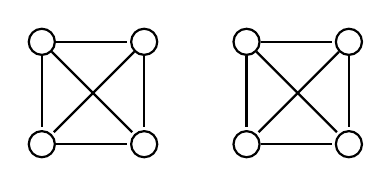
\begin{tikzpicture}[-,>=stealth,shorten >=1pt,auto,node distance=1.3cm, thick,main node/.style={scale=0.9,circle,draw,font=\sffamily\normalsize}]

            \node[circle, draw] (1) []{};
            \node[circle, draw] (2) [right of = 1]{};
            \node[circle, draw] (3) [below of = 1]{};
            \node[circle, draw] (4) [right of = 3]{};

            \node[circle, draw] (5) [right of = 2]{};
            \node[circle, draw] (6) [right of = 5]{};
            \node[circle, draw] (7) [below of = 5]{};
            \node[circle, draw] (8) [right of = 7]{};

            \draw[-] (1) to (2);
            \draw[-] (1) to (3);
            \draw[-] (1) to (4);
            \draw[-] (2) to (3);
            \draw[-] (2) to (4);
            \draw[-] (3) to (4);

            \draw[-] (5) to (6);
            \draw[-] (5) to (7);
            \draw[-] (5) to (8);
            \draw[-] (6) to (7);
            \draw[-] (6) to (8);
            \draw[-] (7) to (8);

            ;
        \end{tikzpicture}
        % \caption{A \tit{matching} of the previous graph.}
        % \label{matching}
    \end{figure}

    composed of two disconnected $K_4$. Here, we have that $$\delta = 4 - 1 = 3 \ge \dfrac{2 \cdot 4}{2} - 1 = 4 - 1 = 3 = \dfrac{n}{2} - 1$$ However, $\delta \ge \tfrac{n}{2} - 1$ is not sufficient to guarantee connectivity.

    \section{Exercises}

    \begin{framedprob}{}
        Let $G = (V, E)$ be a graph of $n$ vertices, where $n \ge 2$. Show that there must be two vertices $x, y \in V$ such that $\deg(x) = \deg(y)$.
    \end{framedprob}

    \solution{
        By definition, the range of the possible degrees for any node of $G$ is $[0, n - 1]$. By way of contradiction, assume that for any two vertices $x, y \in V$ it holds that $\deg(x) \neq \deg(y)$; hence, since the graph has $n$ nodes, it must be that each node is assigned a different degree, and that we use all the possible degrees in $[0, n - 1]$. In particular, this implies that there are two vertices $u, v \in V$ such that $\deg(u) = 0$ and $\deg(v) = n - 1$, but this is a contradiction because if the degree of $v$ is $n - 1$, it must be adjacent to all the other nodes of $V$, including $u$, and $\deg(u) = 0$ $\lightning$.
    }

    \chapter{Matchings}

    \begin{frameddefn}{Matching}
        Given a graph $G = (V, E)$, a \tbf{matching} of $G$ is a set of edges $M \subseteq E$ such that $$\forall e, e' \in M \quad e \cap e' = \varnothing$$
    \end{frameddefn}

    \begin{figure}[H]
        \centering
        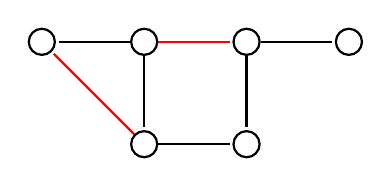
\begin{tikzpicture}[-,>=stealth,shorten >=1pt,auto,node distance=1.3cm, thick,main node/.style={scale=0.9,circle,draw,font=\sffamily\normalsize}]

            \node[circle, draw] (1) []{};
            \node[circle, draw] (2) [right of = 1]{};
            \node[circle, draw] (3) [below of = 1]{};
            \node[circle, draw] (4) [below of = 2]{};
            \node[circle, draw] (5) [left of = 1]{};
            \node[circle, draw] (6) [right of = 2]{};

            \draw[-] (1) [red] to (2);
            \draw[-] (1) to (3);
            \draw[-] (2) to (4);
            \draw[-] (1) to (5);
            \draw[-] (3) to (4);
            \draw[-] (3) [red] to (5);
            \draw[-] (2) to (6);

            ;
        \end{tikzpicture}
        \caption{A \tit{matching} of the previous graph.}
        \label{matching}
    \end{figure}

    As shown in figure, a matching is nothing more than a set of edges that must not share endpoints with each other — for this reason, in literature it is often referred to as \tbf{independent edge set}. 

    Given a matching $M$ in a graph $G$, we say that a vertex $v \in V(G)$ is \tbf{free} w.r.t. $M$ if there are no edges $e \in M$ such that $e \cap v \neq \varnothing$. An edge $xy \in E(G)$ is said to be \tit{disjoint} from $M$ if both $x$ and $y$ are free w.r.t. $M$.

    In graph theory we are often interested in the matching that has the largest possible cardinality of a graph. For this purpose, we often distinguish the two following concepts, namely \tit{maximal} and \tit{maximum} matching.

    \begin{frameddefn}{Maximal matching}
        A \tbf{maximal matching} is a matching that cannot be extended any further.
    \end{frameddefn}
    
    For instance, the matching shown in \cref{matching} is actually a \tbf{maximal matching}, because no other edge in $E$ can be added to che current set of edges $M$ of the matching without breaking the matching condition.

    \begin{frameddefn}{Maximum matching}
        A \tbf{maximum matching} is a matching that has the largest cardinality.
    \end{frameddefn}

    Clearly, the previous example does not repreent a \tbf{maximum matching}, because the following set of edges

     \begin{figure}[H]
        \centering
        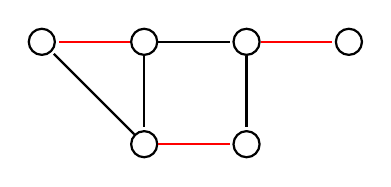
\begin{tikzpicture}[-,>=stealth,shorten >=1pt,auto,node distance=1.3cm, thick,main node/.style={scale=0.9,circle,draw,font=\sffamily\normalsize}]

            \node[circle, draw] (1) []{};
            \node[circle, draw] (2) [right of = 1]{};
            \node[circle, draw] (3) [below of = 1]{};
            \node[circle, draw] (4) [below of = 2]{};
            \node[circle, draw] (5) [left of = 1]{};
            \node[circle, draw] (6) [right of = 2]{};

            \draw[-] (1) to (2);
            \draw[-] (1) to (3);
            \draw[-] (2) to (4);
            \draw[-] (1) [red] to (5);
            \draw[-] (3) [red] to (4);
            \draw[-] (3) to (5);
            \draw[-] (2) [red] to (6);

            ;
        \end{tikzpicture}
    \end{figure}

    is still a valid matching for the graph, but has a larger cardinality than the previous set.

    Given a matching $M$ in a graph $G$, what conditions must be met to increase its cardinality? Trivially, if there exists an edge $e$ disjoint from $M$, clearly $M \cup \{e\}$ is a larger matching than $M$ --- implying that $M$ was not \tit{maximal} in $G$. However, this is not the only situation in which the cardinality of $M$ can be extended. In fact, consider the following definitions.

    \section{Augmenting paths}

    \begin{frameddefn}{Alternating path}
        Given a graph $G$, and a matching $M$ in $G$, an \tbf{$M$-alternating path} is a path of $G$ that starts at a free node w.r.t. $M$, and is composed of edges that alternate between $M$ and $E(G) - M$.
    \end{frameddefn}

    \begin{figure}[H]
        \centering
        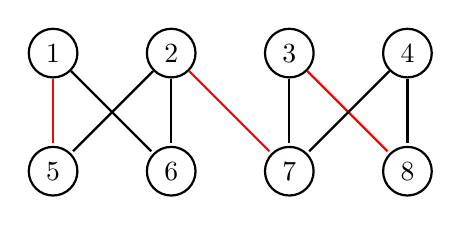
\begin{tikzpicture}[-,>=stealth,shorten >=1pt,auto,node distance=1.5cm, thick,main node/.style={scale=0.9,circle,draw,font=\sffamily\normalsize}]

            \node[circle, draw] (1) []{1};
            \node[circle, draw] (2) [right of = 1]{2};
            \node[circle, draw] (3) [right of = 2]{3};
            \node[circle, draw] (4) [right of = 3]{4};
            \node[circle, draw] (5) [below of = 1]{5};
            \node[circle, draw] (6) [below of = 2]{6};
            \node[circle, draw] (7) [below of = 3]{7};
            \node[circle, draw] (8) [below of = 4]{8};

            \draw[-] (1) [red] to (5);
            \draw[-] (1) to (6);
            \draw[-] (2) to (6);
            \draw[-] (2) to (5);
            \draw[-] (2) [red] to (7);
            \draw[-] (3) to (7);
            \draw[-] (3) [red] to (8);
            \draw[-] (4) to (7);
            \draw[-] (4) to (8);

            ;
        \end{tikzpicture}
        \caption{For instance, if $M$ is the set of \tit{red} edges --- which forms a matching of the graph --- then $6 \ \{6, 2\} \ 2 \ \{2, 7\} \ 7 \ \{7, 3\} \ 3 \ \{3, 8\} \ 8$ is an $M$-alternating path.}
        % \label{}
    \end{figure}
    
    \begin{frameddefn}{Augmenting path}
        Given a graph $G$, and a matching $M$ in $G$, an \tbf{$M$-augmenting path} is an $M$-alternating path that ends at a free vertex w.r.t. $M$.
    \end{frameddefn}

    For example, if we consider the path $$6 \ \{6, 2\} \ 2 \ \{2, 7\} \ 7 \ \{7, 3\} \ 3 \ \{3, 8\} \ 8 \ \{8, 4 \} \ 4$$ this is actually an $M$-augmenting path of the previous graph. Augmenting paths are very useful because they can be used to \tit{expand} the cardinality of an initial matching. In fact, in the previous graph we can actually define a \tit{larger} matching by \tbf{swapping} the edges of this augmenting path, as shown below

    \begin{figure}[H]
        \centering
        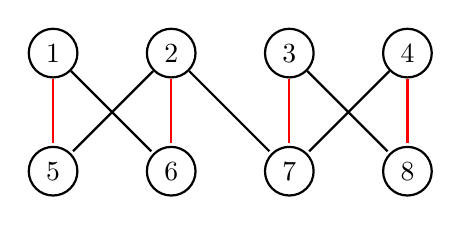
\begin{tikzpicture}[-,>=stealth,shorten >=1pt,auto,node distance=1.5cm, thick,main node/.style={scale=0.9,circle,draw,font=\sffamily\normalsize}]

            \node[circle, draw] (1) []{1};
            \node[circle, draw] (2) [right of = 1]{2};
            \node[circle, draw] (3) [right of = 2]{3};
            \node[circle, draw] (4) [right of = 3]{4};
            \node[circle, draw] (5) [below of = 1]{5};
            \node[circle, draw] (6) [below of = 2]{6};
            \node[circle, draw] (7) [below of = 3]{7};
            \node[circle, draw] (8) [below of = 4]{8};

            \draw[-] (1) [red] to (5);
            \draw[-] (1) to (6);
            \draw[-] (2) [red] to (6);
            \draw[-] (2) to (5);
            \draw[-] (2) to (7);
            \draw[-] (3) [red] to (7);
            \draw[-] (3) to (8);
            \draw[-] (4) to (7);
            \draw[-] (4) [red] to (8);

            ;
        \end{tikzpicture}
        % \caption{For instance, if $M$ is the set of \tit{red} edges --- which forms a matching of the graph --- then $6 \ \{6, 2\} \ 2 \ \{2, 7\} \ 7 \ \{7, 3\} \ 3 \ \{3, 8\} \ 8$ is an $M$-alternating path.}
        % \label{}
    \end{figure}

    \subsection{Berge's theorem}

    This suggests that the presence of augmenting paths in a graph is a \tit{sufficient} condition for a matching \tit{not} to be maximum, but we can actually prove that it is also \tit{necessary}, as stated in the following theorem, proved by \textcite{berge} in 1957.

    \begin{framedthm}[label={aug paths}]{Berge's theorem}
        Given a graph $G$, $M$ is a maximum matching of $G$ if and only if there are no $M$-augmenting paths.
    \end{framedthm}

    \proofiff{
        By contrapositive, consider a graph $G$ and a matching $M$ such that there is an $M$-augmenting path $P$ in $G$. Moreover, by way of contradiction assume that $M$ is maximum; however $M \Delta E(P)$ is a larger matching than $M$ --- here, $\Delta$ is the \href{https://en.wikipedia.org/wiki/Symmetric_difference}{symmetric difference}, therefore the operation $M \Delta E(P)$ has the same effect of \tit{swapping} the edges of $P$ between the ones in $M$ and in $E(P) - M$.
    }{
        By contrapositive, consider a graph $G$ and a matching $M$ of $G$ that is not maximum, i.e. there exists a matching $M^*$ of $G$ such that $\abs M < \abs{M^*}$. Consider the subgraph of $G$ that has the vertices of $V(G)$ and the edges described by $M \Delta M^*$; the symmetric difference of these two sets will yield the set of edges that are either in $M$ or in $M^*$, but not in $M \cap M^*$, therefore this subgraph is \tit{not} a multigraph. Moreover, since $M$ and $M^*$ are both matchings, we have that

        \begin{enumerate}[label={(\arabic*)}]
            \item the degrees of the vertices of this subgraph can be either 0, 1 or 2
            \item in each component of the subgraph the edges \tit{must} alternate between $M$ and $M^*$
        \end{enumerate}

        By the observation (1), we have that each component of the subgraph can be either

        \begin{itemize}
            \item a isolated vertex
            \item a cycle
            \item a path
        \end{itemize}

        and by observation (2), we have that all the cycle components must have \tit{even} length, which implies that they have the same number of edges of $M$ and $M^*$. On the other hand, path components may have either even or odd length; in particular, even-length paths must have the same number of edges of $M$ and $M^*$ --- as for cycle components --- while odd-length paths have a different number of edges of $M$ and $M^*$. However, since $\abs M < \abs{M^*}$, there must be at least one path component of this subgraph such that its edges of $M$ are less than the edges of $M^*$, and this is clearly an $M$-augmenting path.
    }

    Given a graph $G$, and a matching $M$ of $G$, what is the maximum possible value for $\abs M$? To answer this question, we need to introduce the following combinatorial structure.

    \subsection{Kőnig's theorem}

    \begin{frameddefn}{Vertex cover}
        Given a graph $G$, a \tbf{vertex cover} for $G$ is a set of vertices $C \subseteq V(G)$ such that every edge in $G$ is incident to at least one vertex in $C$. Using symbols $$\forall (u, v) \in E(G) \quad u \in C \lor v \in C$$
    \end{frameddefn}

    \begin{figure}[H]
        \centering
        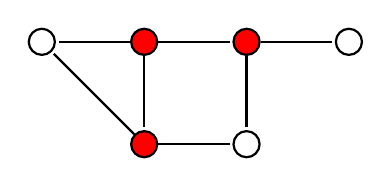
\begin{tikzpicture}[-,>=stealth,shorten >=1pt,auto,node distance=1.3cm, thick,main node/.style={scale=0.9,circle,draw,font=\sffamily\normalsize}]

            \node[circle, draw, fill=red] (1) []{};
            \node[circle, draw, fill=red] (2) [right of = 1]{};
            \node[circle, draw, fill=red] (3) [below of = 1]{};
            \node[circle, draw] (4) [below of = 2]{};
            \node[circle, draw] (5) [left of = 1]{};
            \node[circle, draw] (6) [right of = 2]{};

            \draw[-] (1) to (2);
            \draw[-] (1) to (3);
            \draw[-] (2) to (4);
            \draw[-] (1) to (5);
            \draw[-] (3) to (4);
            \draw[-] (3) to (5);
            \draw[-] (2) to (6);

            ;
        \end{tikzpicture}
        \caption{An example of a vertex cover.}
    \end{figure}
    
    As shown in figure, a vertex cover is simply a set of vertices that must \tit{cover} all the edges of the graph. For vertex covers, we are interested in the \tit{minimum} possible cardinality --- the concepts of \tit{minimal} and \tit{minimum} are defined analogously.

    As introduced before, through vertex covers we can bound the size of any matching of a graph.

    \begin{framedthm}{Matchings bound vertex covers}
        Given a graph $G$, a matching $M$, and a vertex cover $S$ of $G$, it holds that $\abs M \le \abs S$.
    \end{framedthm}

    \begin{proof}
        By definition, any vertex cover $S$ of $G = (V, E)$ is also a vertex cover for $G^B = (V, B)$, for any set of edges $B \subseteq E$, and in particular this is true for $G^M = (V, M)$.

        Now consider $G^M$, and a vertex cover $C$ on it: by construction we have that $\Delta \le 1$, therefore any vertex in $C$ will cover at most 1 edge of $M$. This implies that if $\abs C = k$, then $C$ will cover at most $k$ edges of $G^M$.

        Lastly, since $G^M$ has $\abs M$ edges by definition, any vertex cover defined on $G^M$ has to contain at least $\abs M$ vertices. This implies that no vertex cover $S$ of $G$ smaller than $\abs M$ can exist, because $S$ will have to cover at least the edges in $M$.
    \end{proof}

    \begin{framedcor}{}
        Given a graph $G$, a maximum matching $M^*$ and a minimum vertex cover $S^*$, it holds that $\abs {M^*} \le \abs {S^*}$.
    \end{framedcor}

    Moreover, if the graph is bipartite this theorem is actually \tit{stronger}, as proved by \textcite{konig} in 1931.

    \begin{framedthm}[label={konig}]{Kőnig's theorem}
        Given a bipartite graph $G$, a maximum matching $M^*$ and a minimum vertex cover $S^*$, it holds that $\abs {M^*} = \abs {S^*}$.
    \end{framedthm}

    \begin{proof}
        Consider a graph $G$, a maximum matching $M^*$ and a minimum vertex cover $S^*$ of $G$; by the previous corollary, it follows that to prove the statement it suffices to show that there exists a vertex cover $S$ such that $\abs S = \abs{M^*}$, because $$\abs{M^*} \le \abs{S^*} \le \abs S = \abs{M^*} \implies \abs{M^*} = \abs{S^*}$$ Hence, we are going to construct the following vertex cover. Let $G$ be bipartitioned through $(A, B)$; then, for each edge $ab \in M^*$ such that $a \in A$ and $b \in B$, we place $b \in S$ if and only if there exists an $M^*$-alternating path that starts in $A$ and ends at $b$, otherwise we place $a \in S$.

        \begin{figure}[H]
            \centering
            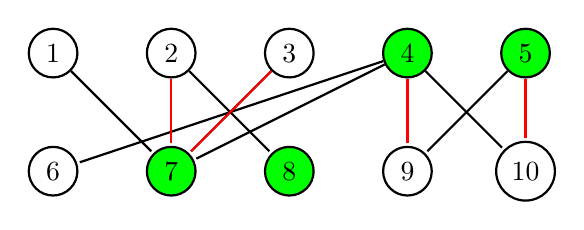
\begin{tikzpicture}[-,>=stealth,shorten >=1pt,auto,node distance=1.5cm, thick,main node/.style={scale=0.9,circle,draw,font=\sffamily\normalsize}]

                \node[circle, draw] (1) []{1};
                \node[circle, draw] (2) [right of = 1]{2};
                \node[circle, draw] (3) [right of = 2]{3};
                \node[circle, draw, fill=green] (4) [right of = 3]{4};
                \node[circle, draw, fill=green] (5) [right of = 4]{5};
                \node[circle, draw] (6) [below of = 1]{6};
                \node[circle, draw, fill=green] (7) [below of = 2]{7};
                \node[circle, draw, fill=green] (8) [below of = 3]{8};
                \node[circle, draw] (9) [below of = 4]{9};
                \node[circle, draw] (10) [below of = 5]{10};

                \draw[-] (1) to (7);
                \draw[-] (2) to (8);
                \draw[-] (3) to (7);
                \draw[-] (4) to (6);
                \draw[-] (4) to (7);
                \draw[-] (4) to (10);
                \draw[-] (5) to (9);

                \draw[-] (2) [red] to (7);
                \draw[-] (3) [red] to (7);
                \draw[-] (4) [red] to (9);
                \draw[-] (5) [red] to (10);

                ;
            \end{tikzpicture}
            \caption{For instance, given this graph bipartitioned into $(A, B)$ --- where $A$ is the uppermost row of vertices --- and the \tit{red} matching, we would construct the \tit{green} vertex cover.}
            % \label{}
        \end{figure}

        Note that, by definition, it holds that $\abs S = \abs{M^*}$.

        \claim{
            $S$ is a vertex cover for $G$.
        }{
            Consider an edge $ab \in E(G)$ such that $a \in A$ and $b \in B$; note that, by definition of $S$ all the edges in $M^*$ are already covered, hence we may assume that $ab \notin M^*$. We have two cases.

            \begin{itemize}
                \item $a$ is free, i.e. $\nexists ab' \in M^*$ for $b' \in B$. Note that $b$ cannot be free, otherwise $M^* \cup \{ab\}$ would still be a matching of $G$ but greater than $M^*$. Hence, there must be an edge $a'b \in M^*$ for some $a' \in A$. Therefore, since $a$ is free, the edge $ab$ is a trivial $M^*$-alternating path ending at $b \in B$, meaning that $b \in S$ by definition, implying that $ab$ is covered by $S$.

                \item $a$ is matched, i.e. $\exists ab' \in M^*$ for $b' \in B$. Therefore, by definition of $S$, either $a$ or $b'$ lies in $S$. In particular, if $a \in S$, then $ab$ is trivially covered by $S$, hence suppose that $b' \in S$.

                    Observe that, by definition of $S$ this implies that there must be an $M^*$-alternating path $P$ that starts in $A$ and ends at $b'$.

                    \begin{itemize}
                        \item If $ab, ab' \notin E(P)$, then $P \cup \{b'a\} \cup ab$ is an $M^*$-augmenting path, which would contradict the fact that $M^*$ is maximum by \cref{aug paths} $\lightning$
                        \item If $ab \notin E(P)$ but $ab' \in E(P)$, then $P$ could not have been an $M^*$-alternating path starting at a vertex in $A$ $\lightning$.
                        \item If $ab \in E(P)$ but $ab' \notin E(P)$, then $P$ must have had the following form $$\ldots \ b'' \ \{b'', a\} \ a \ \{a, b\} \ b \ \{b, a'\} \ a' \ \{a', b'\} \ b'$$ where $a' \in A$, $b'' \in B$. However, since $ab' \in M^*$ and $ab \notin M^*$, and the edges of $P$ must alternate w.r.t. $M^*$, $ab''$ must lie inside $M^*$, contradicting $ab' \in M^*$ by definition of matching $\lightning$.
                    \end{itemize}

                    This implies that $ab', ab \in E(P)$, meaning that $P$ encounters $b$ \curlyquotes{before} $b'$. However, this implies that $P - \{ab'\}$ is an $M^*$-alternating path that starts in $A$ and ends at $b$, thus $b \in S$ by definition, concluding that $ab$ is still covered by $S$.
            \end{itemize}
        }

        Hence, we have constructed a vertex cover $S$ such that $\abs S = \abs{M^*}$, meaning that the statement holds because of the previous observation.
    \end{proof}

    \subsection{Finding maximum matchings}

    Consider a matching $M$ of a graph $G$, and an $M$-augmenting path $P$; the idea of \tit{swapping} the edges of $P$ between $M$ and $E(G) - M$ is very useful when $G$ is \tbf{bipartite}. In fact, we can actually describe a procedure which is able to return a \tit{maximum matching} of a bipartite graph, by swapping the edges of the augmenting paths present in $G$. However, for this algorithm to work, we first need a procedure capable of finding augmenting paths in bipartite graphs, which is defined down below:

    \begin{enumerate}
        \item Assume that the considered graph $G$ is bipartite through $(A, B)$, and consider a matching $M$ of $G$
        \item Starting from a node $a \in A$ free w.r.t. $M$, compute a \tit{modified} BFS such that the edges of its tree alternate between $E(G) - M$ and $M$
        \item If the tree of the BFS contains a free leaf $b \in B$, then the path $v \to b$ is $M$-augmenting
    \end{enumerate}

    For instance, given the following bipartite graph $G$, and a matching $M$ of $G$ --- outlined in \tit{red}

    \begin{figure}[H]
        \centering
        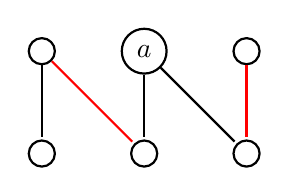
\begin{tikzpicture}[-,>=stealth,shorten >=1pt,auto,node distance=1.3cm, thick,main node/.style={scale=0.9,circle,draw,font=\sffamily\normalsize}]

            \node[circle, draw] (1) []{};
            \node[circle, draw] (2) [right of = 1]{$a$};
            \node[circle, draw] (3) [right of = 2]{};
            \node[circle, draw] (4) [below of = 1]{};
            \node[circle, draw] (5) [right of = 4]{};
            \node[circle, draw] (6) [right of = 5]{};

            \draw[-] (1) to (4);
            \draw[-] (1) [red] to (5);
            \draw[-] (2) to (5);
            \draw[-] (2) to (6);
            \draw[-] (3) [red] to (6);

            ;
        \end{tikzpicture}
        % \caption{An example of a perfect matching.}
    \end{figure}

    the \tit{modified} BFS rooted in $a$ would produce the following tree 

    \begin{figure}[H]
        \centering
        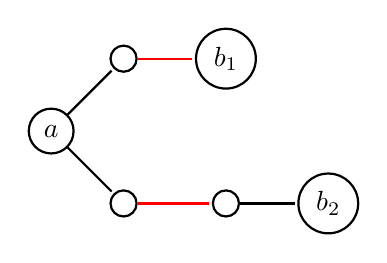
\begin{tikzpicture}[-,>=stealth,shorten >=1pt,auto,node distance=1.3cm, thick,main node/.style={scale=0.9,circle,draw,font=\sffamily\normalsize}]

            \node[circle, draw] (1) []{$a$};
            \node[circle, draw] (2) [above right of = 1]{};
            \node[circle, draw] (3) [right of = 2]{$b_1$};
            \node[circle, draw] (4) [below right of = 1]{};
            \node[circle, draw] (5) [right of = 4]{};
            \node[circle, draw] (6) [right of = 5]{$b_2$};

            \draw[-] (1) to (2);
            \draw[-] (2) [red] to (3);
            \draw[-] (1) to (4);
            \draw[-] (4) [red] to (5);
            \draw[-] (5) to (6);

            ;
        \end{tikzpicture}
        % \caption{An example of a perfect matching.}
    \end{figure}

    and we observe that the path $a \to b_1$ is $M$-alternating, while the path $a \to b_2$ is $M$-augmenting. The next proposition guarantees that if there are $M$-augmenting paths that start in $a$, our \tit{modified} BFS will find at least one of them.

    \begin{framedprop}{}
        Given a bipartite graph $G$, bipartitioned into $(A, B)$, and a matching $M$ of $G$, if there exists an $M$-augmenting path in $G$ that starts in a vertex $a \in A$ free w.r.t. $M$, then there exists an $M$-augmenting path in the tree $T$ of the \tit{modified} BFS.
    \end{framedprop}

    \begin{proof}
        Let $P$ be an $M$-augmenting path that starts in $a$ and minimizes the edges in $E(P) - E(T)$ and, by way of contradiction, assume that $E(P) - E(T) \neq \varnothing$, i.e. $P$ is not completely contained in $T$. Therefore, let $xy$ be the first edge in $E(P) - E(T)$ encountered while traversing $P$, starting at $a$, and without loss of generality assume that $x \in V(P)$.

        \claim{
            $x \in A$.
        }{
            By way of contradiction, assume that $x \in B$.

            \begin{itemize}
                \item Assume that $x$ is not a leaf of $T$. Since the BFS starts at $a \in A$, and the edges of $T$ alternate between $M$ and $E(G) - M$, if $x \in B$ then the next edge $xy'$ in $T$ is an edge in $M$. Moreover --- by the same reasoning --- since $P$ is $M$-augmenting, it must be that $xy \in M$, meaning that $xy, xy' \in M$ contradicting the definition of matching $\lightning$
                \item Now, assume that $x$ is a leaf of $T$. By the same reasoning, $xy$ must be in $M$ because $P$ is $M$-augmenting, but $xy \notin E(T)$ would imply that the BFS stopped before adding the edge $xy$ to $T$ $\lightning$.
            \end{itemize}
        }

        For instance, given the following setting

        \begin{figure}[H]
            \centering
            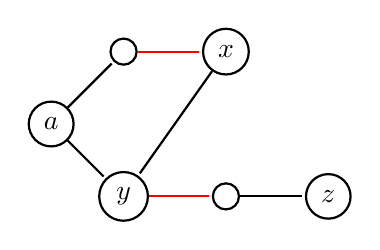
\begin{tikzpicture}[-,>=stealth,shorten >=1pt,auto,node distance=1.3cm, thick,main node/.style={scale=0.9,circle,draw,font=\sffamily\normalsize}]

                \node[circle, draw] (1) []{$a$};
                \node[circle, draw] (2) [above right of = 1]{};
                \node[circle, draw] (3) [right of = 2]{$x$};
                \node[circle, draw] (4) [below right of = 1]{$y$};
                \node[circle, draw] (5) [right of = 4]{};
                \node[circle, draw] (6) [right of = 5]{$z$};

                \draw[-] (1) to (2);
                \draw[-] (2) [red] to (3);
                \draw[-] (1) to (4);
                \draw[-] (4) [red] to (5);
                \draw[-] (5) to (6);
                \draw[-] (3) to (4);

                ;
            \end{tikzpicture}
            % \caption{An example of a perfect matching.}
        \end{figure}

        a possible path for $P$ would be $a \to x \to y \to z$. However, the path $a \to y \to z$ is still an $M$-augmenting path that starts at $a$ but has one fewer edge not in $T$ w.r.t. $P$, contradicting the definition of $P$ $\lightning$.

        Note that, in the general case we would consider the path $P' := a \ T \ y \cup y \ P$, however this is not guaranteed to be a path. The complete proof leverages the fact that $G$ is bipartite in order to prove that $P'$ is indeed a path, but it is very technical and outside the scope of these notes.
    \end{proof}

    Finally, now that we have a procedure which is guaranteed to find an augmenting path in a given bipartite graph, to return a maximum matching it suffices to run the following algorithm.

    \begin{framedalgo}{Maximum matching (bipartite graphs)}
        Given a bipartite graph $G$, the algorithm returns a maximum matching for $G$. \\
        \hrule

        \quad
        \begin{algorithmic}[1]
            \Function{MaximumMatchingBipGraphs}{$G$}
                \State $M := \varnothing$
                \Do
                    \State $P := \textsc{findAugmentingPath}(G)$ \Comment{the previous procedure}
                    \State Swap the edges between $M$ and $E(G) - M$ in $P$
                \doWhile{$P \neq \texttt{None}$}
                \State \textbf{return} $M$
            \EndFunction
        \end{algorithmic}
    \end{framedalgo}

    In particular, the output of this algorithm is guaranteed to be a \tit{maximum} matching thanks to \cref{aug paths}, since the algorithm terminates when there are no more augmenting paths left in the graph $G$.

    \section{Perfect matching}

    By definition, a matching is \tit{not} forced to cover all the vertices of a graph. However, if this happens the matching is called \tbf{perfect matching}.

    \begin{frameddefn}{Perfect matching}
        Given a graph $G$, a \tbf{perfect matching} of $G$ is a matching that covers all the vertices of $G$, i.e. $M$ is a perfect matching if and only if $$\forall v \in V(G) \quad \exists e \in M \quad v \cap e \neq \varnothing$$
    \end{frameddefn}

    \begin{figure}[H]
        \centering
        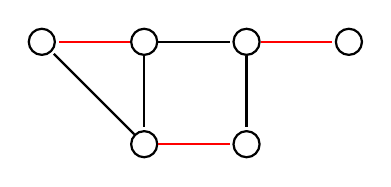
\begin{tikzpicture}[-,>=stealth,shorten >=1pt,auto,node distance=1.3cm, thick,main node/.style={scale=0.9,circle,draw,font=\sffamily\normalsize}]

            \node[circle, draw] (1) []{};
            \node[circle, draw] (2) [right of = 1]{};
            \node[circle, draw] (3) [below of = 1]{};
            \node[circle, draw] (4) [below of = 2]{};
            \node[circle, draw] (5) [left of = 1]{};
            \node[circle, draw] (6) [right of = 2]{};

            \draw[-] (1) to (2);
            \draw[-] (1) to (3);
            \draw[-] (2) to (4);
            \draw[-] (1) [red] to (5);
            \draw[-] (3) [red] to (4);
            \draw[-] (3) to (5);
            \draw[-] (2) [red] to (6);

            ;
        \end{tikzpicture}
        \caption{An example of a perfect matching.}
    \end{figure}

    Perfect matchings are an interesting topic of study when related to \tit{bipartite graphs}. We observe that if a bipartite graph $G$, bipartitioned into $(A, B)$, admits a perfect matching $M$, it must be that $\abs A = \abs B$. This is because every matched edge must connect one vertex from $A$ to one vertex from $B$, and by definition $M$ matched \tit{each} vertex exactly once. However, the converse is not true.

    \begin{figure}[H]
        \centering
        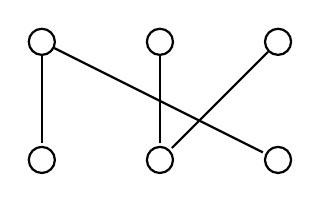
\begin{tikzpicture}[-,>=stealth,shorten >=1pt,auto,node distance=1.5cm, thick,main node/.style={scale=0.9,circle,draw,font=\sffamily\normalsize}]

            \node[circle, draw] (1) []{};
            \node[circle, draw] (2) [right of = 1]{};
            \node[circle, draw] (3) [right of = 2]{};
            \node[circle, draw] (4) [below of = 1]{};
            \node[circle, draw] (5) [below of = 2]{};
            \node[circle, draw] (6) [below of = 3]{};

            \draw[-] (1) to (4);
            \draw[-] (1) to (6);
            \draw[-] (2) to (5);
            \draw[-] (3) to (5);

            ;
        \end{tikzpicture}
        \caption{For instance, this bipartite graph, bipartitioned into $(A, B)$ such that $A$ is the uppermost row of vertices, even if $\abs A = \abs B$ this graph does not admit a perfect matching.}
        % \label{}
    \end{figure}

    \subsection{Hall's theorem}

    Because of this characterization on bipartite graphs, in addition to the concept of \tit{perfect matching}, if $\abs {A} \neq \abs{B}$ we can define a \tit{weaker} version of \curlyquotes{perfect}.

    \begin{frameddefn}{$A$-perfect matching}
        Given a bipartite graph $G$, bipartitioned through $(A, B)$ such that $\abs A \le \abs B$, we say that a matching $M$ is an \tbf{$A$-perfect matching} if it covers all the vertices in $A$.
    \end{frameddefn}

    Note that we can always assume that $\abs A \le \abs B$, without loss of generality. The following theorem, known as the \href{https://en.wikipedia.org/wiki/Hall%27s_marriage_theorem}{Hall's marriage theorem} --- proved by \textcite{hall} in 1935 --- shows the conditions that guarantee that an $A$-perfect matching exists.

        \begin{framedthm}[label={hall}]{Hall's marriage theorem}
        Given a bipartite graph $G$, bipartitioned into $(A, B)$, then $G$ admits an $A$-perfect matching if and only if $$\forall S \subseteq A \quad \abs S \le \abs{\mathcal N (S)}$$
    \end{framedthm}

    \begin{proof}
        The direct implication is trivially true by definition of matching. We will prove the converse implication by contrapositive. Therefore, suppose that the bipartite graph $G$ does not admit any $A$-perfect matching, and consider a minimum vertex cover $V^*$ of $G$. Then, by \cref{konig}, since $G$ is bipartite we know that for any maximum matching $M^*$ of $G$ it holds that $\abs{M^*} = \abs{V^*}$. However, since we are assuming that there are no $A$-perfect matchings of $G$, any maximum matching must have size strictly less than $\abs A$, meaning that $\abs{V^*} = \abs{M^*} < \abs A$.

        Now, consider the set $S := A - V^*$; since $G$ is bipartite, it must hold that $$\mathcal N(S) \subseteq V^* \cap B \implies \abs{\mathcal N(S)} \le \abs{V^* \cap B} = \abs {V^*} - \abs{A \cap V^*}$$ Moreover, observe that $$V^* \cap A = A - (A - V^*) = A - S \implies \abs{V^* \cap A}  = \abs A - \abs S$$ therefore, we have that $$\abs{\mathcal N(S)} \le \abs{V^*} - \abs{V^* \cap A} = \abs{V^*} - \abs A + \abs S$$ Lastly, since $\abs {V^*} < \abs A \iff \abs{V^*} - \abs A < 0$, we conclude that $$\abs{\mathcal N (S)} \le \abs{V^*} - \abs A + \abs S < 0 + \abs S = \abs S \implies \abs{\mathcal N(S)} < \abs S$$ which proves that there is at least one set $S$ for which the \tit{Hall condition} does not hold.
    \end{proof}

    \subsection{Tutte's theorem}

    In the general case, what obstructs the existence of a perfect matching in a graph? Consider a graph $G$; clearly, if $n$ is odd, the graph does not admit perfect matchings, since each edge matches exactly two nodes, meaning that there will always be a free vertex in the graph.

    \begin{figure}[H]
        \centering
        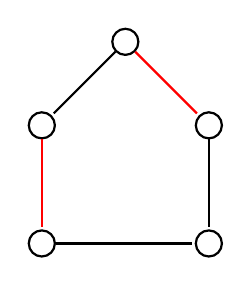
\begin{tikzpicture}[-,>=stealth,shorten >=1pt,auto,node distance=1.5cm, thick,main node/.style={scale=0.9,circle,draw,font=\sffamily\normalsize}]

            \node[circle, draw] (1) []{};
            \node[circle, draw] (2) [below left of = 1]{};
            \node[circle, draw] (3) [below right of = 1]{};
            \node[circle, draw] (4) [below of = 2]{};
            \node[circle, draw] (5) [below of = 3]{};

            \draw[-] (1) to (2);
            \draw[-] (1) [red] to (3);
            \draw[-] (2) [red] to (4);
            \draw[-] (3) to (5);
            \draw[-] (4) to (5);

            ;
        \end{tikzpicture}
        \caption{For instance, no matching of $C_5$ can be perfect.}
    \end{figure}

    For the same reasoning, if $G$ has a connected component with an odd number of vertices, $G$ does not admit perfect matchings. Hence, if $G$ admits a perfect matching, there cannot be any connected component with an odd number of vertices. But is the converse true as well? Consider the following graph

    \begin{figure}[H]
        \centering
        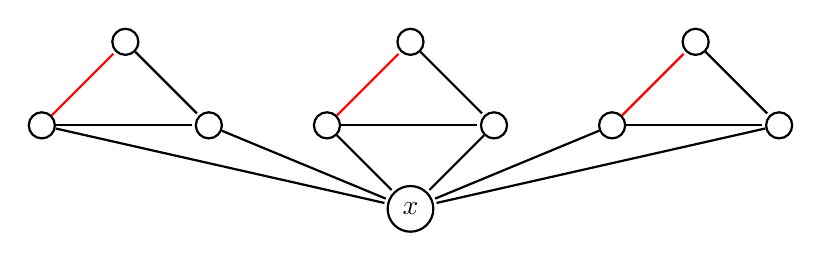
\begin{tikzpicture}[-,>=stealth,shorten >=1pt,auto,node distance=1.5cm, thick,main node/.style={scale=0.9,circle,draw,font=\sffamily\normalsize}]

            \node[circle, draw] (1) []{};
            \node[circle, draw] (2) [above right of = 1]{};
            \node[circle, draw] (3) [below right of = 2]{};
            \node[circle, draw] (4) [right of = 3]{};
            \node[circle, draw] (5) [above right of = 4]{};
            \node[circle, draw] (6) [below right of = 5]{};
            \node[circle, draw] (7) [right of = 6]{};
            \node[circle, draw] (8) [above right of = 7]{};
            \node[circle, draw] (9) [below right of = 8]{};
            \node[circle, draw] (10) [below left of = 6]{$x$};

            \draw[-] (1) [red] to (2);
            \draw[-] (2) to (3);
            \draw[-] (1) to (3);
            \draw[-] (4) [red] to (5);
            \draw[-] (5) to (6);
            \draw[-] (4) to (6);
            \draw[-] (7) [red] to (8);
            \draw[-] (8) to (9);
            \draw[-] (7) to (9);

            \draw[-] (1) to (10);
            \draw[-] (3) to (10);
            \draw[-] (4) to (10);
            \draw[-] (6) to (10);
            \draw[-] (7) to (10);
            \draw[-] (9) to (10);

            ;
        \end{tikzpicture}
        % \caption{For instance, no matching of $C_5$ can be perfect.}
    \end{figure}

    This graph is connected, and has 10 vertices, but it does not admit perfect matchings, meaning that the converse does not hold. Can we find a condition that guarantees that a given graph always admits a perfect matching?

    Given a graph $G$, let $\mathcal O (G)$ be the number of components with an odd number of vertices. The next theorem, proved by \textcite{tutte} in 1947 shows that the following property $$\forall S \subseteq V(G) \quad \mathcal O(G[V(G) - S]) \le \abs S$$ which we will refer to as \tbf{Tutte condition} --- is a \tit{necessary} and \tit{sufficient} condition to guarantee that a graph admits a perfect matching. In fact, in the example of $C_5$ we observe that the set that violates the Tutte condition is $S = \varnothing$, and in the second example is $S = \{x\}$.

    \begin{framedlem}{}
        Given a graph $G$, and a supergraph $G'$ of $G$, if $G$ satisfies the Tutte condition, then $G'$ satisfies the Tutte condition as well.
    \end{framedlem}

    \begin{proof}
        By contrapositive, suppose that $G'$ fails the Tutte condition, meaning that there exists a set $S \subseteq V(G') = V(G)$ such that $\mathcal O (G[V(G') - S]) > \abs S$. Since $G'$ is obtained by adding edges to $G$, the number of odd components in $G'$ can either remain the same, or decrease if two different components having an odd number of vertices became connected in $G'$. Therefore, we have that $$\abs S < \mathcal O (G[V(G') - S]) \le \mathcal O (G[V(G) - S])$$ meaning that $G$ fails the Tutte condition as well.
    \end{proof}

    We are now ready to prove Tutte's theorem.

    \begin{framedthm}{Tutte's theorem}
        A graph $G$ admits a perfect matching if and only if for any $S \subseteq V(G)$ it holds that $\mathcal O(G[V(G) - S]) \le \abs S$ --- meaning that it satisfies the Tutte condition.
    \end{framedthm}

    \proofiff{
        For the direct implication, consider a graph $G$ that admits a perfect matching $M$, and by way of contradiction assume that there exists a set $S \subseteq V(G)$ that violates the Tutte condition. For the previous observation, we know that each component of $G[V(G) - S]$ that has an even number of vertices will not have free nodes w.r.t. $M$, and each component of $G[V(G) - S]$ that has an odd number of vertices will have one free node w.r.t. $M$. In particular, these free vertices must be covered by $M$, since $M$ is perfect, and the only way they can be covered by $M$ is through the vertices of $S$. However, since $\mathcal O (G[V(G) - S]) > \abs S$, there exists at least one free vertex in $G[V(G) - S]$ w.r.t. $M$ that cannot be matched to any of the vertices of $S$, meaning that $M$ is not perfect $\lightning$.
    }{
        We will prove the contrapositive of the converse implication. Therefore, suppose that $G$ does not admit any perfect matching, and we will prove that there exists a set of vertices for which the Tutte condition does not hold. Let $G'$ be the maximal supergraph of $G$ that still does not admit perfect matchings. We say that a set $X$ satisfies the \tit{clique-adjacency} condition if every component of $G'[V(G') - X]$ is a clique, and every vertex $u \in X$ is adjacent to every vertex $v \notin X$.

        \claim{
            If there is a subset $S' \subseteq V(G')$ that satisfies the clique-adjacency condition, then $G$ does not satisfy the Tutte condition.
        }{
            Note that $S' \subseteq V(G') = V(G)$, hence if $S'$ violates the Tutte condition on $G$, the claim is trivially true. Therefore, we will assume that $S'$ satisfies both the clique-adjacency condition, and the Tutte condition on $G$.

            Let $S'$ be a subset that satisfies the clique-adjacency condition; hence, by definition every component of $G'[V(G') - S']$ is a clique. Thus, consider a clique, and let $n$ be the number of its vertices.
            
            \begin{itemize}
                \item If $n$ is even, we can always find a perfect matching restricted on it.
                \item If $n$ is odd, we can always find a perfect matching restricted to $n - 1$ vertices, but since we are assuming that $S'$ satisfies the Tutte condition on $G$, we know that $\mathcal O (G[V(G) - S']) \le \abs {S'}$. Therefore, by the clique-adjacency condition we know that we can always match the $n$-th vertex of the clique with a vertex of $S'$.
            \end{itemize}

            % Note that the free vertices of $S'$ must form a clique as well, otherwise \todo{va visto nel dettaglio il motivo}. 
            TODO \todo{da finire}
        }

        Consider the set $$S := \{v \in V(G') \mid \deg_{G'}(v) = n - 1\}$$ By way of contradiction, suppose that $S$ violates the clique-adjacency condition. This happens if at least one of the following holds:

        \begin{enumerate}[label={(\arabic*)}]
            \item there are two vertices $u \in S$ and $v \notin S$ such that $u \notin S$
            \item there is a component of $G'[V(G') - S]$ that is not a clique
        \end{enumerate}

        However, by definition of $S$, each vertex $v \in S$ has $\deg_{G'} = n - 1$, hence $(1)$ cannot be true, meaning that $(2)$ must hold. Hence, consider a connected component of $G'[V(G') - S]$ that is not a clique, i.e. there are at least two vertices $x$ and $y$ such that $x \nsim y$.

        Let $P$ be the shortest path from $x$ to $y$ in $G'[V(G') - S]$, and let $a$, $b$ and $c$ be the first three vertices of $P$ --- note that $a, b, c \notin S$. We observe that $a \nsim c$, otherwise $P$ would not be the shortest path. Note that $b \notin S$, therefore $\deg_{G'}(b) < n - 1$, i.e. there exists a vertex $d$ such that $b \nsim d$.

        \begin{figure}[H]
            \centering
            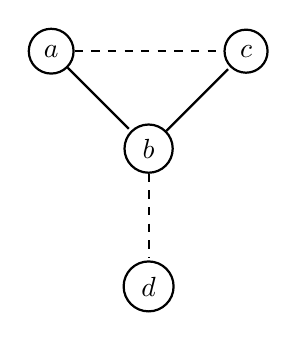
\begin{tikzpicture}[-,>=stealth,shorten >=1pt,auto,node distance=1.75cm, thick,main node/.style={scale=0.9,circle,draw,font=\sffamily\normalsize}]

                \node[circle, draw] (1) []{$a$};
                \node[circle, draw] (2) [below right of = 1]{$b$};
                \node[circle, draw] (3) [above right of = 2]{$c$};
                \node[circle, draw] (4) [below of = 2]{$d$};

                \draw[-] (1) to (2);
                \draw[-] (2) to (3);
                \draw[dashed] (1) to (3);
                \draw[dashed] (2) to (4);

                ;
            \end{tikzpicture}
            \caption{The \curlyquotes{kite-shaped} figure we are considering --- the dashed lines represent the \tit{missing edges}.}
        \end{figure}

        By maximality of $G'$, we know that $G' \cup \{ac\}$ must have a perfect matching $M_1$, and $G' \cup \{bd\}$ must have a perfect matching $M_2$. Moreover, $ac \in M_1$ and $bd \in M_2$, otherwise $M_1$ and $M_2$ would be perfect matchings on $G'$.

        \claim{
            $(M_1 - \{ac\}) \cup (M_2 - \{bd\})$ contains a perfect matching for $G'$.
        }{
            Let $\overline M = (M_1 - \{ac\}) \Delta (M_2 - \{bd\})$. By the same reasoning applied for \cref{aug paths}, since $M_1$ and $M_2$ are two matchings, every vertex of $\overline M$ has degree at most 2. Hence, consider a vertex $z$ in the subgraph induced by $\overline M$

            \begin{itemize}
                \item if $\deg_{\overline M}(z)$ is 0 or 2, $z$ is matched both by $M_1$ and $M_2$
                \item since $M_1$ is a perfect matching, each vertex of $G'$ is matched by $M_1 - \{ac\}$, except for $a$ and $c$
                \item likewise, since $M_2$ is a perfect matching, each vertex of $G'$ is matched by $M_2 - \{bd\}$, except for $b$ and $d$
            \end{itemize}

            which implies that the only vertices $z$ that have $\deg_{\overline M}(z) = 1$ are precisely $a$, $b$, $c$ and $d$.

            Moreover, each component of the subgraph induced by $\overline M$ is either an isolated vertex, a cycle or a path, and the edges of the components must alternate between $M_1$ and $M_2$. Therefore, because of the degrees of $a$, $b$, $c$ and $d$, it must be that these vertices are endpoints of two alternating paths $P_1$ and $P_2$. Moreover, since $ac \in M_1$ and $bd \in M_2$, one of these paths must be an $M_1$-alternating path, while other must be $M_2$ alternating --- and without loss of generality let $P_1$ be the $M_1$-alternating. Note that the set $$M' := (M_1 \cup M_2) - (E(P_1) \cup E(P_2))$$ is a perfect matching on $G[V(G) - (V(P_1) \cup V(P_2))]$. We have three cases for $P_1$ and $P_2$:

            \begin{enumerate}
                \item $P_1$ is a path $a \to c$, and $P_2$ is a path $b \to d$; then $$(M_1 \cap E(P_2)) \cup (M_2 \cap E(P_1)) \cup M'$$ is a perfect matching on $G'$
                \item $P_1$ is a path $a \to b$, and $P_2$ is a path $c \to d$; then $$(M_1 \cap E(P_2)) \cup (M_2 \cap E(P_1)) \cup M' \cup \{bd\}$$ is a perfect matching on $G'$
                \item $P_1$ is a path $a \to d$, and $P_2$ is a path $b \to c$; then $$(M_1 \cap E(P_2)) \cup (M_2 \cap E(P_1)) \cup M' \cup \{ac\}$$ is a perfect matching on $G'$
            \end{enumerate}
        }

        Therefore, because of this claim $G'$ always contains a perfect matching, contradicting the definition of $G'$. This implies that $S$ must satisfy the clique-adjacency condition. Hence, by the first claim we have that $G$ satisfies the Tutte condition \todo{first claim is wrong?}
    }

    \section{Stable matching}

    Matchings in bipartite graphs are particularly useful as they can be applied to model various types of problems across different fields. One well-known example is the \href{https://en.wikipedia.org/wiki/Stable_marriage_problem}{stable matching problem}, which arises in scenarios like job assignments, college admissions, and matchmaking systems. In this problem, the goal is to find a \tit{stable pairing} between two sets of entities --- such as students and universities --- where no two unmatched entities would prefer each other over their current assignments.

    \begin{frameddefn}{Stable matching}
        Given a graph $G$, bipartitioned through $(A, B)$, and a matching $M$ of $G$, consider a family of \tit{preference} functions $\{w_v\}_{v \in V(G)}$ that for each vertex $v \in V(G)$, assign a value to the edges $vu \in E(G)$, for all $u \in \mathcal N (v)$ $$\forall v \in V(G) \quad \func{w_v}{\mathcal N (v)}{\R}$$ We say that $M$ is \tbf{stable} if for each $ab \in E(G)$ it does \underline{not} happen that $$(a \ \mathrm{free} \ \lor (\exists ab' \in M \quad w_a(b) > w_a(b')))$$ $$\land$$ $$(b \ \mathrm{free} \ \lor (\exists a'b \in M \quad w_b(a) > w_b(a')))$$
    \end{frameddefn}

    For instance, consider the following bipartite graph $G$, and a matching $M$ --- outlined in \tit{red}:

    \begin{figure}[H]
        \centering
        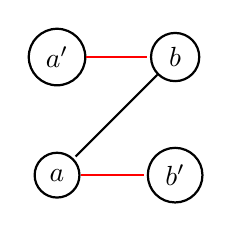
\begin{tikzpicture}[-,>=stealth,shorten >=1pt,auto,node distance=1.5cm, thick,main node/.style={scale=0.9,circle,draw,font=\sffamily\normalsize}]

            \node[circle, draw] (1) []{$a'$};
            \node[circle, draw] (2) [right of = 1]{$b$};
            \node[circle, draw] (3) [below of = 1]{$a$};
            \node[circle, draw] (4) [below of = 2]{$b'$};

            \draw[-] (1) [red] to (2);
            \draw[-] (2) to (3);
            \draw[-] (3) [red] to (4);

            ;
        \end{tikzpicture}
        % \caption{For instance, this bipartite graph, bipartitioned into $(A, B)$ such that $A$ is the uppermost row of vertices, even if $\abs A = \abs B$ this graph does not admit a perfect matching.}
        % \label{}
    \end{figure}

    If the family of preference functions $\{w_v\}_{v \in V}$ is such that $$w_a(b) > w_b(b') \land w_b(a) > w_b(a')$$ which implies that \underline{both} $a$ and $b$ would prefer to \tit{switch} their current matched vertex --- then $M$ is \tit{not} stable. Note that the empty matching is \tit{not} stable, by definition.

    The following theorem, proved by \textcite{gale} in 1962, proves that a stable matching can be always constructed in a bipartite graph, regardless of the preference functions.

    \begin{framedthm}{Gale-Shapley theorem}
        Given a bipartite graph $G$, and a family of preference functions $\{w_v\}_{v \in V(G)}$, there exists a stable matching of $G$.
    \end{framedthm}

    \begin{proof}
        Before proving the theorem, we need to introduce some definitions.

        Consider a bipartite graph $G$, bipartitioned through $(A, B)$, and consider a matching $M$. Given two vertices $a \in A$ and $b \in B$, we say that $a$ is \tbf{acceptable to $b$} if

        \begin{itemize}
            \item $b$ is free, or
            \item $b$ is matched to a vertex $a'$, and $w_b(a) > w_b(a')$
        \end{itemize}

        Moreover, we say that a vertex $a \in A$ is \tbf{happy} if either
        
        \begin{itemize}
            \item $a$ is free, or
            \item $ab \in M$ and for each $b'$ such that $a$ is acceptable to $b'$, it holds that $w_a(b) \ge w_a(b')$
        \end{itemize}

        Observe that in the empty matching every vertex is happy.

        \claim{
            Consider a matching $M$ such that each vertex is happy; if $M$ is not stable, then there exists a vertex $a \in A$ such that $a$ is free and acceptable to some $b \in B$.
        }{
            By instability of $M$, there must be an edge $ab \notin M$ such that $a$ is free, or it prefers $b$ to its current partner, and vice versa. By way of contradiction, suppose that $a$ is matched to some $b' \in B$, hence by instability of $M$ through $ab$ we know that $w_a(b) > w_a(b')$

            \begin{itemize}
                \item If $b$ is free, then by definition $a$ is acceptable to $b$; however, by happiness of $a$ it must be that $w_a(b') \ge w_a(b)$ $\lightning$
                \item If $b$ is matched by some edge $a'b \in M$, by instability of $M$ through $ab$ we know that $w_b(a) > w_b(a')$, hence $a$ is acceptable to $b$, and by happiness of $a$ it must be that $w_a(b') \ge w_a(b)$ $\lightning$
            \end{itemize}

            This implies that $a$ must be free; therefore, we have that

            \begin{itemize}
                \item If $b$ is free as well, then by definition $a$ is acceptable to $b$
                \item If $b$ is matched by some edge $a'b \in M$, by instability of $M$ through $ab$ we know that $w_b(a) > w_b(a')$, hence $a$ is still acceptable to $b$
            \end{itemize}
        }

        Now, consider another matching $M'$ of $G$; we say that $M$ is \tbf{better than $M'$} if 

        \begin{itemize}
            \item $\forall a'b \in M' \quad \exists ab \in M \quad w_b(a) \ge w_b(a')$, meaning that every vertex $b \in B$ prefers its match in $M$ at least as much as its match in $M'$, and
            \item $\exists a'b \in M', ab \in M \quad w_b(a) > w_b(a')$, meaning that there is at least one vertex $b$ that strictly perfers its match in $M$ over its match in $M'$
        \end{itemize}
        
        In other words, $M$ is better than $M'$ if no match in $M$ is worse than in $M'$, and at least one match is strictly better.

        Let $M_k$ be an unstable matching such that every vertex is happy; therefore, by the previous claim we know that there exists a vertex $a \in A$ such that $a$ is free and and acceptable to some $b \in B$. We will construct a matching $M_{k + 1}$ as follows: $$b^* \in \argmax_{\substack{b \in \mathcal N (a) : \\ a \ \mathrm{acceptable \ to} \ b}}{w_a(b)} \implies M_{k + 1} := (M_k \cup \{ab^*\}) - \{a'b^* \in M_k \mid a' \in A\}$$ meaning that $M_{k + 1}$ is obtained from $M_k$ by adding the edge $ab^*$, where $b^*$ maximizes $w_a(b^*)$, and removing the edge $a'b^*$ from $M_k$, if present --- the last set is either $\{a'b^*\}$ or $\varnothing$.

        \claim{
            $M_{k + 1}$ is better than $M_k$, and if $M_k$ is ensures that every vertex is happy, $M_{k +1}$ does as well.
        }{
            First, we prove that $M_{k +1}$ is better than $M_k$. The first condition that $M_{k +1}$ has to satisfy in order to be better than $M_k$ is true simply because we removed the edge $a'b^*$ if it was present in $M_k$, and the rest of the matching has not been altered. Moreover, if $b^*$ was free then the second condition is vacuously true, otherwise if the edge $a'b^*$ was present in $M_k$, in $M_{k +1}$ there we added the edge $ab^*$ and we know that $w_{b^*}(a) > w_{b^*}(a')$ because $a$ is acceptable to $b^*$ by definition.

            Now, assume that $M_k$ is such that every vertex is happy. Since $b^*$ is the neighbor of $a$ that maximizes $w_a(b^*)$, $a$ is happy by definition. Now, if $b^*$ was free in $M_k$, then we only added $ab^*$ to $M_{k + 1}$, hence every vertex is happy w.r.t. $M_{k + 1}$. Otherwise, if $b^*$ was not free in $M_k$, i.e. there was an edge $a'b^* \in M_k$, by definition $M_{k + 1}$ will not contain $a'b^*$, meaning that $a'$ is free w.r.t. $M_{k +1}$, hence $a'$ is happy by definition.
        }

        Now, consider the empty matching $M_0 := \varnothing$; we already observed that $M_0$ is not stable, but is such that each vertex is happy, therefore by the previous claim we can extend $M_0$ into $M_1$ through some vertex $a \in A$ that satisfied the condition of the first claim. In particular, since we proved that this process preserves the happiness of the vertices, we can repeat this process as long as the current matching $M_i$ is still unstable.

        Observe that every matching in the sequence is better than the previous ones, therefore such sequence cannot cycle. Moreover, since there is a finite number of possible matching of $G$, the sequence will eventually reach a matching where every vertex of $A$ is matched --- if $\abs A \neq \abs B$ we can assume that $\abs A < \abs B$ without loss of generality; call this matching $\hat M$. Hence, by contrapositive of the first claim, we know that $\hat M$ is either unstable, or has an unhappy vertex. However, by construction of our sequence, every vertex of $\hat M$ is happy, therefore it must be that $\hat M$ is stable.
    \end{proof}

    \section{Exercises}

    \begin{framedprob}{}
        Let $G$ be a $k$-regular bipartite graph, bipartitioned through $(A, B)$. Prove that

        \begin{enumerate}
            \item $\abs A = \abs B$
            \item $G$ has a perfect matching
        \end{enumerate}
    \end{framedprob}

    \begin{proof}
        Since $G$ is $k$-regular, it holds that the number of edges that have an endpoint in $A$ is precisely $k \abs A$, and the number of edges that have an endpoint in $B$ is exactly $k \abs B$; moreover, since $G$ is bipartite, we have that $$k \abs A = k \abs B \implies \abs A = \abs B$$

        We will prove the second statement by using \cref{hall}. By way of contradiction, assume that there is a set $S \subseteq V(G)$ such that $\abs S > \abs{\mathcal N(S)} \implies k \abs S > k \abs{\mathcal N (S)}$. Applying the same argument as before, the number of edges $ab$ such that $a \in S, b \in \mathcal N (S)$ is exactly $k \abs S$, hence by the pigeonhole principle there must be at least one vertex in $\mathcal N (S)$ that has more than $k$ vertices, contradicting the $k$-regularity of $G$.
    \end{proof}

    \chapter{TODO}

    TODO \todo{introduction}
    
    \begin{frameddefn}{$A$-$B$ paths}
        Given a graph $G$, and two sets $A, B \subseteq V(G)$, an \tbf{$A$-$B$ path} is a path that has one end in $A$, one end in $B$, and no internal vertices in $A \cup B$.
    \end{frameddefn}

    \begin{figure}[H]
        \centering
        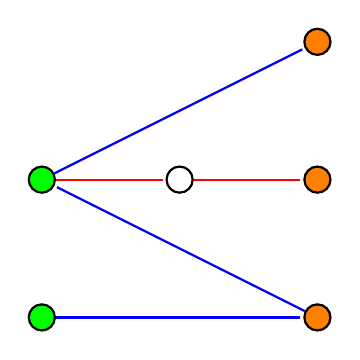
\begin{tikzpicture}[-,>=stealth,shorten >=1pt,auto,node distance=1.75cm, thick,main node/.style={scale=0.9,circle,draw,font=\sffamily\normalsize}]

            \node[circle, draw, fill=green] (1) []{};
            \node[circle, draw] (2) [right of = 1]{};
            \node[circle, draw, fill=orange] (3) [right of = 2]{};
            \node[circle, draw, fill=green] (4) [below of = 1]{};
            \node[circle, draw, fill=orange] (5) [below of = 3]{};
            \node[circle, draw, fill=orange] (6) [above of = 3]{};

            \draw[-] (1) [red] to (2);
            \draw[-] (2) [red] to (3);
            \draw[-] (4) [blue] to (5);
            \draw[-] (5) [blue] to (1);
            \draw[-] (1) [blue] to (6);

            ;
        \end{tikzpicture}
        \caption{For instance, if $A$ is the set of \tit{green} vertices, and $B$ is the set of \tit{orange} vertices, then the \tit{red} is an $A$-$B$ path but the \tit{blue} one is not.}
        % \label{first graph}
    \end{figure}

    Note that if $A \cap B \neq \varnothing$, any vertex in $A \cap B$ is a trivial $A$-$B$ path.

    \begin{frameddefn}{$A$-$B$ hitting set}
        Given a graph $G$, and two sets $A, B \subseteq V(G)$, an \tbf{$A$-$B$ hitting} set is a set $X \subseteq V(G)$ such that every $A$-$B$ path has a vertex in $X$.
    \end{frameddefn}

    \begin{figure}[H]
        \centering
        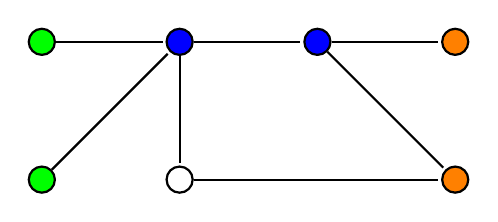
\begin{tikzpicture}[-,>=stealth,shorten >=1pt,auto,node distance=1.75cm, thick,main node/.style={scale=0.9,circle,draw,font=\sffamily\normalsize}]

            \node[circle, draw, fill=green] (1) []{};
            \node[circle, draw, fill=blue] (2) [right of = 1]{};
            \node[circle, draw, fill=blue] (3) [right of = 2]{};
            \node[circle, draw, fill=orange] (4) [right of = 3]{};
            \node[circle, draw] (5) [below of = 2]{};
            \node[circle, draw, fill=green] (6) [below of = 1]{};
            \node[circle, draw, fill=orange] (7) [below of = 4]{};

            \draw[-] (1) to (2);
            \draw[-] (2) to (3);
            \draw[-] (3) to (4);
            \draw[-] (2) to (5);
            \draw[-] (6) to (2);
            \draw[-] (5) to (7);
            \draw[-] (3) to (7);

            ;
        \end{tikzpicture}
        \caption{For example, if $A$ is the set of \tit{green} vertices, and $B$ is the set of \tit{orange} vertices, then the \tit{blue} is an $A$-$B$ hitting set.}
        % \label{first graph}
    \end{figure}

    Note that if $X$ is an $A$-$B$ hitting set, then $A \cap B \subseteq X$, otherwise any single vertex in $A \cap B$ would represent an $A$-$B$ trivial path that does not pass through the hitting set $X$. Moreover, consider an $A$-$B$ hitting set $X$ of a graph $G$; by definition, all the $A$-$B$ paths must have at least one vertex in $X$, but since $A$-$B$ paths do not have internal vertices in $A \cup B$, there cannot be $\abs X + 1$ disjoint $A$-$B$ paths.

    \begin{frameddefn}{$A$-$B$ separation}
        Given a graph $G$, and two sets $A, B \subseteq V(G)$, two sets $X, Y \subseteq V(G)$ describe a \tbf{separation $(X, Y)$} of $G$ if and only if

        \begin{itemize}
            \item $A \subseteq X$
            \item $B \subseteq Y$
            \item $X \cup Y = V(G)$
            \item no edge has one end in $X - Y$ and the other in $Y - X$
        \end{itemize}
 
        We say that a separation $(X, Y)$ has \tbf{order} $\abs{X \cap Y}$.
    \end{frameddefn}

    Given a graph $G$, two sets $A, B \subseteq V(G)$, and an $A$-$B$ separation of $G$, we observe that $G[V(G)-(X \cap Y)]$ is disconnected.

    \begin{framedprop}[label={menger prop}]{}
        Given a graph $G$, and two sets $A, B \subseteq V(G)$, there exists an $A$-$B$ hitting set of size $k$ in $G$ if and only if there exists an $A$-$B$ separation of order $k$.
    \end{framedprop}

    \begin{proof}
        The converse implication is trivially true, because if $(X, Y)$ is an $A$-$B$ separation of $G$, then $X \cap Y$ itself is an $A$-$B$ hitting set of $G$ by definition; therefore, we just need to prove the direct implication.
        
        Let $Z$ be an $A$-$B$ hitting set of $G$ such that $\abs Z = k$, and consider the connected components $C_1, \ldots, C_\ell$ of $G[V(G) - Z]$. Note that there cannot be any component $C_i$ that has a vertex $a \in V(G) \cap (A - Z)$ and a vertex $b \in V(C) \cap (B - Z)$, because otherwise by connectivity of $C_i$ there would be a path $a \to b$ --- which is an $A$-$B$ path --- that avoids the hitting set $Z$. Hence, we can define the two following sets $$X := Z \cup \bigcup_{\substack{C \ \mathrm{component} \\ \mathrm{of} \ G[V(G) - Z] \\ \ \mathrm{such \ that} \ A \cap C \neq \varnothing}}{V(C)}$$ $$Y := Z \cup \bigcup_{\substack{C \ \mathrm{component} \\ \mathrm{of} \ G[V(G) - Z] \\ \mathrm{such \ that} \ A \cap C = \varnothing}}{V(C)}$$ We observe that, by definition

        \begin{itemize}
            \item $A \subseteq X$
            \item $Y$ contains all the vertices in $B - Z$, therefore if $B \cap Z = \varnothing$ then trivially $B \subseteq Y$, and if $B \cap Z \neq \varnothing$ we observe that $Z \subseteq Y$ by definition, hence $B$ is always completely covered by $Y$
            \item $X \cap Y = Z$
        \end{itemize}

        and for the previous observation there cannot be edges with one end in $X - Y$ and the other in $Y - X$. Hence, we conclude that $(X, Y)$ is a separation of $G$, and $X \cap Y = Z \implies \abs{X \cap Y} = \abs Z = k$.
    \end{proof}

    The following theorem establishes a deep connection between \tit{connectivity} and \tit{separation} in graphs, and was proved by \textcite{menger} in 1927.

    \begin{framedthm}[label={menger}]{Menger's theorem}
        Given a graph $G$, and two sets $A, B \subseteq V(G)$, the number of disjoint $A$-$B$ paths is equal to the minimum order of an $A$-$B$ separation of $G$.
    \end{framedthm}

    \proofind{
        Consider an $A$-$B$ separation $(X, Y)$ of minimum order of $G$, i.e. a separation that minimizes $\abs{X \cap Y}$; observe that each $A$-$B$ path must traverse at least one vertex of $X \cap Y$, therefore the number of disjoint $A$-$B$ paths that can exist is at most $\abs{X \cap Y}$. This proves the direct implication of the theorem.

        To prove the converse implication, we would need to prove that the minimum order of an $A$-$B$ separation of $G$ is no more than the number of disjoint $A$-$B$ paths. Instead, we will prove that, for a fixed value $k$, in $G$ there are $k$ disjoint $A$-$B$ paths, or there is an $A$-$B$ separation of order at most $k - 1$, which is logically equivalent. In particular, we will proceed by induction on $m$, i.e. the number of edges of $G$.
    }{
        If $m = 0$, the only possible $A$-$B$ paths in $G$ are trivial paths, i.e. isolated vertices in $A \cap B$. Hence, if $\abs{A \cap B} \ge k$ the base case holds; instead, if $\abs{A \cap B} \le k - 1$, we observe that $A \cap B$ itself is an $A$-$B$ hitting set of $G$ of size at most $k - 1$, which means that there exists an $A$-$B$ separation of order at most $k - 1$ by \cref{menger prop}.
    }{
        Assume that the statement holds on a graph that has $m - 1$ edges.
    }{
        We will prove that the statement holds for a graph $G$ that has $m$ edges as well. In particular, fix an edge $xy \in E(G)$, and note that the graph $G - \{xy\}$ has $m - 1$ edges, meaning that the inductive hypothesis holds for $G - \{xy\}$. However, if $G - \{xy\}$ has $k$ disjoint $A$-$B$ paths, then $G$ also has $k$ disjoint $A$-$B$ paths, therefore we may assume that the inductive hypothesis holds for $G - \{xy\}$ precisely because the latter has an $A$-$B$ separation of order at most $k - 1$.

        Hence, let $(X, Y)$ be an $A$-$B$ separation of $G - \{xy\}$ of order at most $k - 1$; we observe that if $x, y \in X$, or $x, y \in Y$, then $(X, Y)$ is also a separation for $G$, which would conclude the proof. Thus, suppose that $x \in X - Y$ and $y \in Y - X$; then $(X, Y \cup \{x\})$ is an $A$-$B$ separation of $G$ that either has still order at most $k - 1$, or it becomes a separation of order $k$ with $k - 1$ $A$-$B$ paths. Since the first case concludes the proof, we may assume the second one to hold.

        Consider the induced subgraphs $G[X]$ and $G[Y]$ \todo{da finire}
    }

    \section{$k$-connectivity}

    \begin{frameddefn}{$k$-connectivity}
        A graph $G$ is said to be \tbf{$k$-connected} if $\abs{V(G)} \ge k + 1$, and for each $X \subseteq V(G)$ such that $\abs X \le k - 1$ it holds that $G[V(G) - X]$ is connected.
    \end{frameddefn}

    In other words, a graph is $k$-connected if it has at least $k + 1$ vertices, and it remains connected whenever fewer than $k$ vertices are removed.

    \begin{figure}[H]
        \centering
        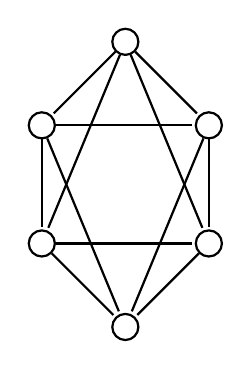
\begin{tikzpicture}[-,>=stealth,shorten >=1pt,auto,node distance=1.5cm, thick,main node/.style={scale=0.9,circle,draw,font=\sffamily\normalsize}]

            \node[circle, draw] (1) []{};
            \node[circle, draw] (2) [below left of = 1]{};
            \node[circle, draw] (3) [below right of = 1]{};
            \node[circle, draw] (4) [below of = 2]{};
            \node[circle, draw] (5) [below of = 3]{};
            \node[circle, draw] (6) [below right of = 4]{};

            \draw[-] (1) to (2);
            \draw[-] (1) to (3);
            \draw[-] (1) to (4);
            \draw[-] (1) to (5);
            \draw[-] (2) to (3);
            \draw[-] (2) to (6);
            \draw[-] (2) to (4);
            \draw[-] (3) to (6);
            \draw[-] (3) to (5);
            \draw[-] (4) to (5);
            \draw[-] (4) to (6);
            \draw[-] (5) to (6);

            ;
        \end{tikzpicture}
        \caption{A 4-connected graph.}
    \end{figure}

    Clearly, any connected graph is 1-connected; moreover, any $K_{t +1}$ clique is $t$-connected.

    \begin{framedprop}[label={kconn}]{}
        If $G$ is $k$-connected, then $\delta \ge k$.
    \end{framedprop}

    \begin{proof}
        By way of contradiction, assume that $\delta < k$, i.e. there is a vertex $x \in V(G)$ such that $\deg(x) < k \implies \abs{\mathcal N(x)} < k$. However, this violates the $k$-connectivity of $G$, because $G[V(G) - \mathcal N (x)]$ is disconnected even though $\abs{\mathcal N(x)} \le k - 1$ $\lightning$.
    \end{proof}

    \begin{framedprop}[label={k-1 conn}]{}
        If $G$ is $k$-connected, then for any $xy \in E(G)$ it holds that $G - \{xy\}$ is $(k - 1)$-connected.
    \end{framedprop}

    \begin{proof}
        By way of contradiction, suppose that $G - \{xy\}$ is not $(k - 1)$-connected, i.e. there exists a set $X \subseteq V(G)$ such that $\abs X \le k - 2$ and $(G - \{xy\})[V(G) - X]$ is disconnected. By $k$-connectivity of $G$, since $\abs X \le k - 2$, we know that $G[V(G) - X]$ is connected, therefore if $(G - \{xy\})[V(G) - X]$ is disconnected it must imply that by removing $xy$ we disconnect $G[V(G) - X]$. Now, since $\abs X \le k - 2$, we know that $\abs{X \cup \{y\}} \le k - 1$, but $G[V(G) - (X \cup \{y\})]$ does not contain the edge $xy$, hence it is disconnected, contradicting the $k$-connectivity of $G$ $\lightning$.
    \end{proof}

    \begin{frameddefn}{Internal disjointness}
        Given a graph $G$, two paths $P_1$ and $P_2$ of $G$ are said to be \tbf{internally disjoint} if every vertex of $V(P_1) \cap V(P_2)$ is an endpoint of $P_1$ and $P_2$.
    \end{frameddefn}

    \begin{figure}[H]
        \centering
        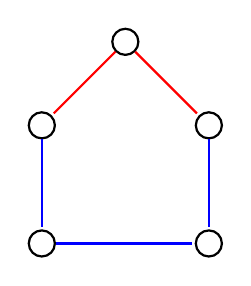
\begin{tikzpicture}[-,>=stealth,shorten >=1pt,auto,node distance=1.5cm,thick,main node/.style={scale=0.9,circle,draw,font=\sffamily\normalsize}]

            \node[circle, draw] (1) []{};
            \node[circle, draw] (2) [below left of = 1]{};
            \node[circle, draw] (3) [below right of = 1]{};
            \node[circle, draw] (4) [below of = 2]{};
            \node[circle, draw] (5) [below of = 3]{};

            \draw[-] (1) [red] to (2);
            \draw[-] (1) [red] to (3);
            \draw[-] (2) [blue] to (4);
            \draw[-] (3) [blue] to (5);
            \draw[-] (4) [blue] to (5);

            ;
        \end{tikzpicture}
        \caption{For instance, the \tit{red} and \tit{blue} paths are internally disjoint.}
    \end{figure}

    \begin{framedprop}{}
        Given a $k$-connected graph, and two sets $A, B \subseteq V(G)$, if $\abs A, \abs B \ge k$ then there exist $k$ disjoint $A$-$B$ paths in $G$.
    \end{framedprop}

    \begin{proof}
        By way of contradiction, if $G$ does not admit $k$ disjoint $A$-$B$ paths, therefore by \cref{menger} the minimum order of an $A$-$B$ separation is at most $k - 1$; hence, let $(X, Y)$ be a minimum order $A$-$B$ separation of $G$, i.e. $\abs{X \cap Y} \le k - 1$. Observe that $\abs{A} \ge k$ and $A \subseteq X$, therefore $\abs X \ge k$ which means that $X - Y \neq \varnothing$, and analogously $Y - X \neq \varnothing$. However, by definition of $A$-$B$ separation we observe that $G[V(G)-(X \cap Y)]$ is disconnected, and we removed less than $k$ vertices, contradicting the $k$-connectivity of $G$ $\lightning$.
    \end{proof}

    \begin{framedprop}[label={intern disj menger}]{}
        Given a $k$-connected graph, for any pair of vertices $x, y \in V(G)$ such that $x \neq y$ there exist $k$ $\{x\}$-$\{y\}$ internally disjoint paths.
    \end{framedprop}

    \begin{proof}
        Fix a pair of distinct vertices $x, y \in V(G)$; we have two cases.

        \begin{itemize}
            \item The two vertices are not adjacent, i.e. $x \nsim y$. By \cref{kconn}, we know that $\abs{\mathcal N(x)} , \abs{\mathcal N(y)} \ge k$, hence by the previous proposition we there exist $k$ disjoint $\mathcal N(x)$-$\mathcal N(y)$ paths, which will form $k$ \tit{internally disjoint} $\{x\}$-$\{y\}$ paths along with the edges to $x$ and $y$.
            \item The two vertices are not adjacent, i.e. $x \nsim y$. By $k$-connectivity of $G$, we know that $G - \{xy\}$ is $(k-1)$-connected by \cref{k-1 conn}, therefore by the same argument of the previous case we have $k - 1$ internally disjoint $\{x\}$-$\{y\}$ path, therefore $G$ will have $k$ internally disjoint $\{x\}$-$\{y\}$ paths along with the edge $xy$.
        \end{itemize}
    \end{proof}

    \begin{framedcor}[label={menger cor}]{}
        Given a $k$-connected graph $G$, a vertex $x \in V(G)$, and a subset $Y \subseteq V(G)$ such that $\abs Y \ge k$, there exist $k$ $\{x\}$-$Y$ paths $P_1, \ldots, P_k$ such that $P_i \cap P_j = \{x\}$ --- for all $i, j \in [k]$ such that $i \neq j$.
    \end{framedcor}

    \begin{proof}
        Add a vertex $z$ to the vertices of $G$, and for each $y \in Y$ add an edge $yz$; we observe that $G[V(G) \cup \{z\}]$ is still $k$-connected, because $\abs Y \ge k$. Now, since $x \neq z$, by the previous proposition there exist $k$ $\{x\}$-$\{z\}$ internally disjoint paths, and these paths must traverse $Y$, therefore each path $P_i$ must have the form $x \to y_i \to z$ for some $y_i \in Y$. Hence, if we consider the subpaths $x \to y_i$ for each $i$, in $G$ these are precisely $k$ $\{x\}$-$Y$ paths intersects only in $x$.
    \end{proof}

    \begin{framedthm}{}
        Given a $k$-connected graph $G$ such that $k \ge 2$, and $k$ vertices $x_1, \ldots, x_k \in V(G)$, there exist a cycle in $G$ that contains all the vertices $x_1, \ldots, x_k$.
    \end{framedthm}
    
    \begin{proof}
        By way of contradiction, let $C$ be the cycle that contains as many vertices $x_i$ as possible; if $x_1, \ldots, x_k \in V(C)$, the theorem is trivially verified, hence we may assume that at least one vertex $x_i$ is not in $V(C)$, and without loss of generality assume that $x_k \notin V(C)$. By \cref{kconn} we know that $\delta \ge k$, and by \cref{min deg 2} we know that $\abs{V(C)} \ge k + 1$. Hence, by the previous corollary we know that exist $k$ $\{x_k\}$-$V(C)$ paths that only intersect in $x_k$.

        Now, since there are at most $k - 1$ vertices $x_i$ in $V(C)$, and there are $k$ $\{x_k\}$-$V(C)$ paths, by the pigeonhole principle there must be a subpath $Q$ of $C$ of the form $x_i \to x_j$ --- for $i, j \in [k - 1]$ distinct --- that has no internal vertex in $\{x_1, \ldots, x_{k - 1}\}$, and such that there are two paths $P_1$ and $P_2$ that $x_k$ as one endpoint and the other lies in $Q$.

        \begin{figure}[H]
            \centering
            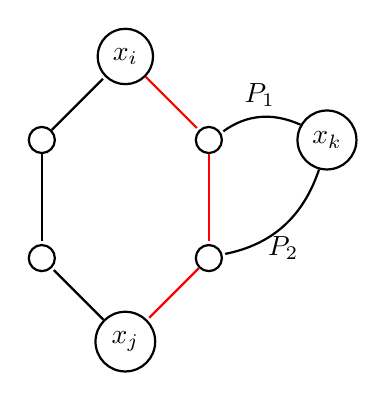
\begin{tikzpicture}[-,>=stealth,shorten >=1pt,auto,node distance=1.5cm,thick,main node/.style={scale=0.9,circle,draw,font=\sffamily\normalsize}]

                \node[circle, draw] (1) []{};
                \node[circle, draw] (2) [above right of = 1]{$x_i$};
                \node[circle, draw] (3) [below right of = 2]{};
                \node[circle, draw] (4) [below of = 3]{};
                \node[circle, draw] (5) [below left of = 4]{$x_j$};
                \node[circle, draw] (6) [above left of = 5]{};
                \node[circle, draw] (7) [right of = 3]{$x_k$};

                \draw[-] (1) to (2);
                \draw[-] (2) [red] to (3);
                \draw[-] (3) [red] to (4);
                \draw[-] (4) [red] to (5);
                \draw[-] (5) to (6);
                \draw[-] (1) to (6);

                \draw[-] (7) [bend right] to node[above]{$P_1$} (3);
                \draw[-] (7) [bend left] to node[below]{$P_2$} (4);

                ;
            \end{tikzpicture}
            \caption{In the figure, the \tit{red} segments compose the subpath $Q$.}
        \end{figure}

        Therefore, we can reroute $Q$ by passing through $P_1$ and $P_2$ in order to find a cycle $C \cup \{x_k\}$ that has a larger number of vertices $x_i$, contradicting the definition of $C$ $\lightning$.
    \end{proof}

    Note that this theorem \tit{does not} guarantee the order in which the vertices are present in the cycle. In fact, asking to preserve the order of the vertices $x_1, \ldots, x_k$ given is a \tit{much harder} question, and the only result we currently know is the following.

    \begin{framedthm}{}
        Given a $10k$-connected graph $G$, and $k$ vertices $x_1, \ldots, x_k \in V(G)$, there exist a cycle in $G$ that contains all the vertices $x_1, \ldots, x_k$ in the same order.
    \end{framedthm}

    \section{Feedback vertex set}

    Consider the following combinatorial structure.

    \begin{frameddefn}{Feedback vertex set}
        Given a graph $G$, a subset $X \subseteq V(G)$ is said to be a \tbf{feedback vertex set} (FVS) if $G[V(G) - X]$ is acyclic; equivalently, $X$ is an FVS if it intersects all cycles of $G$.
    \end{frameddefn}

    \begin{figure}[H]
        \centering
        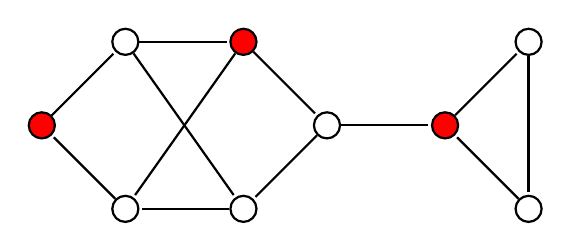
\begin{tikzpicture}[-,>=stealth,shorten >=1pt,auto,node distance=1.5cm,thick,main node/.style={scale=0.9,circle,draw,font=\sffamily\normalsize}]

            \node[circle, draw] (1) []{};
            \node[circle, draw, fill=red] (2) [right of = 1]{};
            \node[circle, draw] (3) [below right of = 2]{};
            \node[circle, draw] (4) [below left of = 3]{};
            \node[circle, draw] (5) [left of = 4]{};
            \node[circle, draw, fill=red] (6) [above left of = 5]{};

            \node[circle, draw, fill=red] (7) [right of = 3]{};
            \node[circle, draw] (8) [above right of = 7]{};
            \node[circle, draw] (9) [below right of = 7]{};

            \draw[-] (1) to (2);
            \draw[-] (2) to (3);
            \draw[-] (3) to (4);
            \draw[-] (4) to (5);
            \draw[-] (5) to (6);
            \draw[-] (6) to (1);

            \draw[-] (3) to (7);
            \draw[-] (7) to (8);
            \draw[-] (8) to (9);
            \draw[-] (9) to (7);

            \draw[-] (1) to (4);
            \draw[-] (2) to (5);

            ;
        \end{tikzpicture}
        \caption{For instance, the \tit{red} set of vertices is an FVS of this graph.}
    \end{figure}

    In many applications, it is important to find a \tbf{minimum} FVS; however, this problem is known to be \NPComplete --- as proved by \textcite{karp} in 1972. Therefore, we often focus on estimating the size of this set by computing lower and upper bounds. In particular, in this section we will present a result proved by \textcite{erdos} in 1965. But before introducing their result about FVSs, we must discuss some combinatorial structures first.

    \subsection{Topological minors}

    Consider a graph $G$, and an edge $xy \in E(G)$; to \tbf{subdivide} $xy$ means to \tit{remove} the edge $xy$ from $E(G)$ and \tit{replacing} with a 2-edge path $x \ z \ y$ for some new vertex $z$. For instance, if $G$ contains the edge $xy$

    \begin{figure}[H]
        \centering
        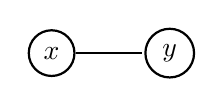
\begin{tikzpicture}[-,>=stealth,shorten >=1pt,auto,node distance=1.5cm,thick,main node/.style={scale=0.9,circle,draw,font=\sffamily\normalsize}]

            \node[circle, draw] (1) []{$x$};
            \node[circle, draw] (2) [right of = 1]{$y$};

            \draw[-] (1) to (2);

            ;
        \end{tikzpicture}
    \end{figure}

    to \tit{subdivide} the edge $xy$ means to replace $xy$ in $G$ with the following 2-edge path

    \begin{figure}[H]
        \centering
        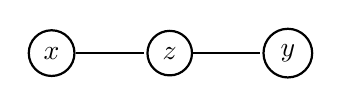
\begin{tikzpicture}[-,>=stealth,shorten >=1pt,auto,node distance=1.5cm,thick,main node/.style={scale=0.9,circle,draw,font=\sffamily\normalsize}]

            \node[circle, draw] (1) []{$x$};
            \node[circle, draw] (2) [right of = 1]{$z$};
            \node[circle, draw] (3) [right of = 2]{$y$};

            \draw[-] (1) to (2);
            \draw[-] (2) to (3);

            ;
        \end{tikzpicture}
    \end{figure}

    \begin{frameddefn}{Subdivision}
        Given a graph $G$, a \tbf{subdivision} of $G$ is a graph obtained from $G$ by repeatedly subdividing its edges.
    \end{frameddefn}

     \begin{figure}[H]
        \centering

        \begin{tabular}{ccc}
            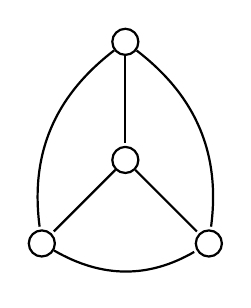
\begin{tikzpicture}[-,>=stealth,shorten >=1pt,auto,node distance=1.5cm,thick,main node/.style={scale=0.9,circle,draw,font=\sffamily\normalsize}]

                \node[circle, draw] (1) []{};
                \node[circle, draw] (2) [below of = 1]{};
                \node[circle, draw] (3) [below left of = 2]{};
                \node[circle, draw] (4) [below right of = 2]{};

                \draw[-] (1) to (2);
                \draw[-] (1) [bend right] to (3);
                \draw[-] (1) [bend left] to (4);
                \draw[-] (2) to (3);
                \draw[-] (2) to (4);
                \draw[-] (3) [bend right] to (4);

                ;
            \end{tikzpicture}

            &\qquad\qquad\qquad&

            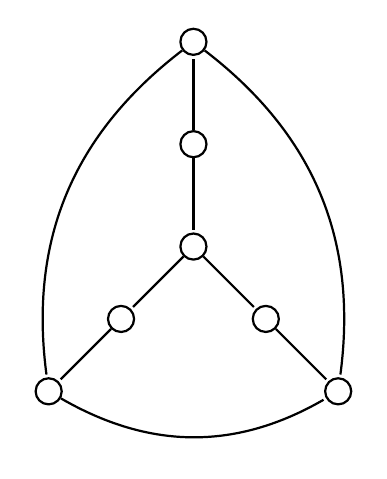
\begin{tikzpicture}[-,>=stealth,shorten >=1pt,auto,node distance=1.3cm, thick,main node/.style={scale=0.9,circle,draw,font=\sffamily\normalsize}]

                \node[circle, draw] (1) []{};
                \node[circle, draw] (2) [below of = 1]{};
                \node[circle, draw] (3) [below left of = 2]{};
                \node[circle, draw] (4) [below right of = 2]{};
                \node[circle, draw] (5) [above of = 1]{};
                \node[circle, draw] (6) [below left of = 3]{};
                \node[circle, draw] (7) [below right of = 4]{};

                \draw[-] (1) to (2);
                \draw[-] (5) [bend right] to (6);
                \draw[-] (5) [bend left] to (7);
                \draw[-] (2) to (3);
                \draw[-] (2) to (4);
                \draw[-] (1) to (5);
                \draw[-] (3) to (6);
                \draw[-] (4) to (7);
                \draw[-] (6) [bend right] to (7);

                ;
            \end{tikzpicture}
        \end{tabular}

        \caption{On the left: $K_4$. On the right: a subdivision of $K_4$.}
    \end{figure}

    Trivially, any graph is a subdivision of itself.

    \begin{frameddefn}{Topological minor}
        Given a graph $G$, and a graph $H$, we say that $G$ contains $H$ as a \tbf{topological minor} if $G$ has a subgraph which is a subdivision of $H$.
    \end{frameddefn}

    \begin{figure}[H]
        \centering
        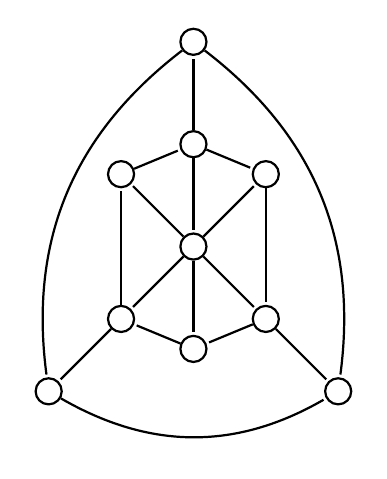
\begin{tikzpicture}[-,>=stealth,shorten >=1pt,auto,node distance=1.3cm, thick,main node/.style={scale=0.9,circle,draw,font=\sffamily\normalsize}]

            \node[circle, draw] (1) []{};
            \node[circle, draw] (2) [below of = 1]{};
            \node[circle, draw] (3) [below left of = 2]{};
            \node[circle, draw] (4) [below right of = 2]{};
            \node[circle, draw] (5) [above of = 1]{};
            \node[circle, draw] (6) [below left of = 3]{};
            \node[circle, draw] (7) [below right of = 4]{};
            \node[circle, draw] (8) [above left of = 2]{};
            \node[circle, draw] (9) [above right of = 2]{};
            \node[circle, draw] (10) [below of = 2]{};

            \draw[-] (1) to (2);
            \draw[-] (5) [bend right] to (6);
            \draw[-] (5) [bend left] to (7);
            \draw[-] (2) to (3);
            \draw[-] (2) to (4);
            \draw[-] (1) to (5);
            \draw[-] (3) to (6);
            \draw[-] (4) to (7);
            \draw[-] (6) [bend right] to (7);
            \draw[-] (2) to (8);
            \draw[-] (2) to (9);
            \draw[-] (2) to (10);

            \draw[-] (8) to (1);
            \draw[-] (1) to (9);
            \draw[-] (9) to (4);
            \draw[-] (4) to (10);
            \draw[-] (10) to (3);
            \draw[-] (3) to (8);

            ;
        \end{tikzpicture}
        \caption{For instance, this graph has $K_4$ as topological minor, because it contains a subdivision of $K_4$ as subgraph.}
    \end{figure}

    \begin{framedthm}{}
        If $G$ is 3-connected, then $G$ has $K_4$ as topological minor.
    \end{framedthm}

    \begin{proof}
        If $G$ is 3-connected, then by \cref{kconn} we know that $\delta_G \ge 3$, and by \cref{min deg 2} this means that in $G$ there is a cycle $C$. Moreover, by 3-connectivity of $G$, we know that $G$ cannot be a cycle itself, therefore there must be at least one vertex $v \notin V(C)$. Now, by 3-connectivity agin we can apply \cref{menger cor}, obtaining 3 $\{v\}$-$V(C')$ paths $P_1$, $P_2$ and $P_3$ that only intersect in $v$, and finally $G[V(C) \cup V(P_1) \cup V(P_2) \cup V(P_3)]$ is a subdivision of $K_4$.
    \end{proof}

    \subsection{Erdős-Pósa theorem}

    \begin{framedprop}{}
        If $G$ is 3-regular multigraph, then $G$ has a cycle of length at most $2 \ceil{\log n}$.
    \end{framedprop}

    \begin{proof}
        Clearly, if $G$ admits loops or parallel edges, the statement is trivially true, therefore we may assume that $G$ is a simple graph.

        Fix a vertex $v \in V(G)$, and grow a BFS tree $T$ from $x$ as long no cycles of length at most $2 \ceil{\log n}$ are encountered. Since $G$ is 3-regular, $T$ will be a tree in which the root $x$ has 3 children, and all the other nodes that are not leaves will have 2 children. If the BFS stopped before visiting all the vertices of $G$, the statement holds, so we may assume that $T$ covers all $V(G)$.

        By 3-regularity of $G$, we have that

        \begin{itemize}
            \item $\delta \ge 3$, hence by \cref{min deg 2} we know that $G$ must contain a cycle
            \item the only possible cycle that can be formed in $G$ is by connecting two leaves of $T$ through an edge
        \end{itemize}

        and lastly, since $V(T) = V(G) = n$, the height of $T$ is $\ceil{\log n} - 1$, which means that such a cycle must have length $$\ceil{\log n} - 1 + \ceil{\log n} - 1 + 1 = 2 \ceil{\log n} - 1$$
    \end{proof}

    Along with the \tit{subdivision} operation that we introduced previously, it naturally follows to defined the \tit{inverse} operation of the subdivision, i.e. the \tbf{suppression}. Given a graph $G$, and two edges $xz, zy \in E(G)$ such that $\deg(z) = 2$, to \tit{suppress} $z$ means to \tit{remove} the vertex $z$ from $V(G)$ along with the edges $xz$ and $zy$, and \tit{replacing} them with an edge $xy$ in $E(G)$. For instance, if $G$ contains the edges $xz$ and $zy$

    \begin{figure}[H]
        \centering
        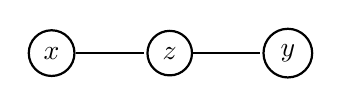
\begin{tikzpicture}[-,>=stealth,shorten >=1pt,auto,node distance=1.5cm,thick,main node/.style={scale=0.9,circle,draw,font=\sffamily\normalsize}]

            \node[circle, draw] (1) []{$x$};
            \node[circle, draw] (2) [right of = 1]{$z$};
            \node[circle, draw] (3) [right of = 2]{$y$};

            \draw[-] (1) to (2);
            \draw[-] (2) to (3);

            ;
        \end{tikzpicture}
    \end{figure}

    to \tit{suppress} the vertex $z$ means to replace $xz$ and $zy$ in $G$ with the following edge $xy$

    \begin{figure}[H]
        \centering
        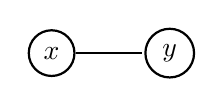
\begin{tikzpicture}[-,>=stealth,shorten >=1pt,auto,node distance=1.5cm,thick,main node/.style={scale=0.9,circle,draw,font=\sffamily\normalsize}]

            \node[circle, draw] (1) []{$x$};
            \node[circle, draw] (2) [right of = 1]{$y$};

            \draw[-] (1) to (2);

            ;
        \end{tikzpicture}
    \end{figure}

    Now, consider the following definition.

    \begin{frameddefn}{Cut}
        Given a graph $G$, and a subset $S \subseteq V(G)$, a the \tbf{cut} induced by $S$ is defined as follows $$\mathrm{cut}(S) := \{e \in E(G) \mid \abs{S \cap e} = 1\}$$
    \end{frameddefn}

    In other words, a \tit{cut} induced by a set $S$ of vertices is the set of edges that have exactly one endpoint in $S$.

    \begin{figure}[H]
        \centering
        \begin{tikzpicture}[-,>=stealth,shorten >=1pt,auto,node distance=1.5cm,thick,main node/.style={scale=0.9,circle,draw,font=\sffamily\normalsize}]

            \node[circle, draw] (1) []{};
            \node[circle, draw, fill=red] (2) [right of = 1]{};
            \node[circle, draw] (3) [below of = 1]{};
            \node[circle, draw, fill=red] (4) [right of = 3]{};
            \node[circle, draw] (5) [left of = 1]{};

            \draw[-] (1) [green] to (2);
            \draw[-] (2) to (4);
            \draw[-] (1) to (3);
            \draw[-] (3) [green] to (4);
            \draw[-] (1) to (5);
            \draw[-] (3) to (5);

            ;
        \end{tikzpicture}
        \caption{For instance, if the set $S$ is described by the \tit{red} vertices, then $\mathrm{cut}(S)$ is the set of green edges.}
    \end{figure}

    We will use the definition of cut in order to prove the following lemma.

    \begin{framedlem}{}
        Given a 3-regular graph $H$ such that $\abs{V(H)} \ge c'k \log (k +1)$ for some constant $c'$, then $H$ contains $k$ disjoint cycles.
    \end{framedlem}

    \proofind{
        We proceed by induction on $k$.
    }{
        For $k = 1$, if $H$ is 3-regular then $\delta_H = 3$, therefore by \cref{min deg 2} it must contain a cycle.
    }{
        Assume that the statement holds for $k - 1$.
    }{
        Let $C$ be a cycle of $H$, and consider the graph $H - C$ --- note that we are \tit{not} considering the induced subgraph $H[V(H) - V(C)]$, but we are just removing the edges of $C$ from $H$.

        \claim{
            $H - C$ has a 3-regular graph $H'$ as topological minor, such that $\abs{V(H')} \ge \abs{V(H)}- 2\abs{V(C)}$.
        }{
            Starting with $V := V(C)$, as long as $H[V(H) - V]$ contains vertices of degree at most 1, move them into $V$; let $M$ be the number of moved vertices. Then, since we are adding vertices to $V$, we have that $\abs{\mathrm{cut}(V)} \le \abs{\mathrm{cut}(C)} - M$. We observe that, by construction $\delta_{H[V(H)- V]} \ge 2$, and the number of vertices that have degree 2 in $H[V(H) - V]$ is at most $\abs{\mathrm{cut}(V)} \le \abs{\mathrm{cut}(C)} - M$.

            Lastly, let $H'$ be the graph obtained from $H[V(H) - V]$ by suppressing all the vertices of degree 2; then we have that $H'$ contains at least the vertices of $H$, without the vertices of $C$, the $M$ vertices that we moved during the procedure, and the vertices of degree 2 that we suppressed. In other words, we have that $$\abs{V(H')} \ge \abs{V(H)} - \abs{V(C)} - M - (\abs{\mathrm{cut}(C)}-M) \ge \abs{V(H)} - 2\abs{V(C)}$$ Note that the last inquality comes from the observation that $\abs{\mathrm{cut}(C)} \le \abs{V(C)}$, which follows by 3-regularity of $H$

            Finally, since $H'$ is 3-regular by construction, and $H[V(H) - V]$ is a subdivision of $H'$ that is contained in $H - C$, this concludes the claim.
        }

        Now, since $\abs{V(H)} \ge c'k \log(k + 1)$, and by the previous proposition we know that $$\abs{V(C)} \le 2 \log (\abs{V(H)}) + 2 \iff - 2 \abs{V(C)} \ge - 4 \log (\abs{V(H)}) - 4$$ where the added term 2 takes care of the rounding error from the ceiling operation --- we obtain the following
        \begin{equation*}
            \begin{split}
                \abs{V(H')} &\ge \abs{V(H)} - 2\abs{V(C)} \\
                            &\ge \abs{V(H)} - 4 \log (\log{V(H)}) - 4 \\
                            &\ge c'k \log (k +1) - 4 \log (c'k \log (k + 1)) - 4 \\
                            &\ge c'k \log (k + 1) - 4[ \log c' + \log k + \log(\log(k + 1))] - 4
            \end{split}
        \end{equation*}

        which is at least $c'(k - 1) \log k$ for sufficiently big values of $c'$. In particular, since $\abs{V(H')} \ge c' (k - 1) \log k$, and we know that $H'$ is 3-regular, we can apply the inductive hypothesis on $H'$, which means that $H'$ contains $k - 1$ disjoint cycles.

        Finally, if $H'$ contains $k$ disjoint cycles, and $H - C$ has $H'$ as topological minor, i.e. $H - C$ contains a subdivision $H''$ of $H'$, by definition of the subdivision operation $H''$ will contain $k -1$ disjoint cycles as well. Therefore, since $H - C$ contains $H''$, $H$ contains $k$ disjoint cycles along with the cycle $C$.
    }

    We are now ready to prove the theorem that we introduced at the beginning of this section.

    \begin{framedthm}{Erdős-Pósa theorem}
        There is a constant $c$ such that for any graph $G$, and any $k \in \N$

        \begin{itemize}
            \item either $G$ has $k$ vertex-disjoint cycles or
            \item there is an FVS $X$ of $G$ such that $\abs X \le c k\log k$
        \end{itemize}
    \end{framedthm}

    \begin{proof}
        If $G$ contains $k$ disjoint cycles, the theorem is trivially true, hence we may assume that $G$ does not have $k$ disjoint cycles. Fix $H$ to be the larget subgraph of $G$ such that $\forall v \in V(H) \quad 2 \le \deg_H(v) \le 3$ --- note that $H$ always exists because we may assume that $G$ contains at least 1 cycle, since if $G$ is acyclic the theorem is trivially true (and we would pick the cycle as $H$ itself). Moreover, fix $\overline H$ to be the subgraph of $G$ without all the \curlyquotes{cycle components} of $G$ --- i.e. components of $G$ that are cycles --- and let $U := \{v \in V(\overline H) \mid \deg_{\overline H}(v) = 3\}$.

        By TODO \todo{discrepanze lemma} we know that $\abs{U} < c'k\log(k + 1)$, for some constant $c$. Let $W$ be a set of vertices composed of one vertex for each cycle component --- the ones not present in $\overline H$.

        \claim{
            Every cycle of $G$ is in $H$.
        }{
            If there was a cycle of $G$ not present in $H$, this cycle would have contained vertices of degree at least 2, contradicting the maximality of $H$.
        }

        \tbf{Claim:} There are no paths $P$ in $G[V(G) - (U \cup W)]$ of length at least 1 such that

        \begin{itemize}
            \item both ends of $P$ are in $H[V(H) - (U \cup W)]$
            \item no internal vertex of $P$ is in $H$
            \item no edge of $P$ is in $H$
        \end{itemize}

        \proofenv[Proof of the Claim]{
            If such a path $P$ exists, then $H \cup P$ is a bigger graph than $H$ that has every vertex of degree 2 or 3, contradicting the maximality of $H$.
        }

        \claim{
            Every cycle of $G - (U \cup W)$ intersects $H$ in exactly one vertex.
        }{
            TODO \todo{da finire}
        }

        TODO \todo{da finire}
    \end{proof}

    \section{Exercises}
    
    \begin{framedprob}
        Given a $k$-connected graph $G$ such that $V(G) \ge 2k$, show that $G$ contains a cycle of length at least 2k.
    \end{framedprob}

    \solution{
        TODO \todo{da fare}
    }

    \printbibliography % UNCOMMENT FOR BIBLIOGRAPHY

\end{document}
